\documentclass[journal,outdir=./]{IEEEtran}
\ifCLASSINFOpdf
  \usepackage[pdftex]{graphicx}
  \usepackage{caption}
  \usepackage[algo2e,ruled,vlined,linesnumbered]{algorithm2e}
  \usepackage{subcaption}
  \usepackage{adjustbox}
  \usepackage{makecell}
  \usepackage{multirow}
  \usepackage{flushend}
  \usepackage{array}
  \usepackage{enumerate}
  \usepackage{hyperref}
  \usepackage{threeparttable}
  \usepackage{epstopdf}
  \usepackage{enumitem}
  \usepackage{xcolor}
  \usepackage{amsmath,amsthm,amssymb}
  \usepackage{bm}
  \usepackage{booktabs}
  \DeclareGraphicsExtensions{.pdf,.png}
\else
  \usepackage[dvips]{graphicx}
  \usepackage{hyperref}
  \DeclareGraphicsExtensions{.eps}
\fi
\usepackage{cite}
\newtheorem{theorem}{Theorem}
\newtheorem{result}{Result}
\newtheorem{proposition}{Proposition}
\newtheorem{lemma}{Lemma}
\newtheorem{corollary}{Corollary}
\newtheorem{remark}{Remark}
\newcommand{\Kr}{K_{\mathrm{reach}}}
\newcommand{\Kc}{K_{\mathrm{commute}}}
\newcommand{\rmax}{r_{\max}}
\newcommand{\rc}{r_{c}}
\newcommand{\Pbar}{\bar{P}}
\newcommand{\Pf}{P_{f}}
\newcommand{\Ph}{P_{h}}
\newcommand{\Emax}{E_{\max}}
\newcommand{\Eu}{E_{u}}
\newcommand{\Gam}{\Gamma}
\newcommand{\Psicap}{\Psi}
\newcommand{\Ru}{R_u}
\newcommand{\todo}[1]{\textcolor{red}{[#1]}}

\hypersetup{hidelinks}
\begin{document}

\title{Fleet Sizing and Coordinated Trajectory Planning\\ for Continuous Age-of-Information Data Collection\\ with UAV Swarms}

\author{Harshvir~\todo{Surname},
        \todo{Advisor Name}, \IEEEmembership{Member, IEEE}
\thanks{H.~\todo{Surname} is with \todo{Department, University, City, Country} (e-mail: \todo{email}).
\par \todo{Advisor} is with \todo{affiliation}.}}

\maketitle

\begin{abstract}
A fleet of $K$ unmanned aerial vehicles (UAVs) operates continuously from a central depot to collect data from $M$ ground sensors, minimising the time-average priority-weighted age of information (AoI) under a fixed fleet-level energy inventory---a fixed total modular battery capacity divided among however many UAVs are flown. How many UAVs should be airborne? We derive a two-regime fleet-sizing rule with no fitted constant: a \emph{reach} cap set by the farthest sensor, which we show duty cycling cannot evade but only relocates to the airborne count; and a \emph{commute} cap set by the realised commute radius, whose governing principle---maximise the fleet's visit rate, proportional to $C/\bar c$---follows exactly from a cost-weighted square-root allocation of visit frequencies under regular visits, a separable long-run marginal-cost model, and a $K$-invariant normalised marginal-cost profile, and whose closed form is a first-order approximation that we show underpredicts in an identified high-budget regime. A closed-form boundary, $\rmax/\rc=1+\sqrt{\Pbar/\Pf}$, predicts which cap binds, and an analytical pre-deployment criterion, computable from the same inputs, flags fields in which the reach cap may not govern within the operating window. On 240 simulated deployments across three layout families, four sensor counts and three budgets, its closed-form point predictor matches the swept optimum to within one UAV in 77\% of instances, and estimating its commute inputs before deployment, from the site survey and known system parameters without a pilot flight or fleet sweep, leaves all 272 point predictions and regime classifications unchanged; where the criterion passes, the median AoI regret of using the rule instead of a sweep is zero; in the clustered (paper) family the 90th percentile is 5\%, and no passing reach-bound instance in any family loses more than $27\%$. Fleet coordination through shared route commitments proves essential: without it, 35--71\% of visits land on sensors another UAV has just served and the objective is $2.9\times$ worse at $K=4$, the rule's fleet size in 9 of the 12 instances. The optimum is more stable across planners than the objective is: an age-blind tour patrol lies within one UAV of our planner's optimum in 92\% of 216 paired deployments although their AoI differs by up to 25\% depending on the layout, and in a controlled comparison with a CP-SAT planner that proves $96.6\%$ of its decisions optimal, all three planners lie within one UAV of each other and of the point predictor in every instance. Under a published $k$-means clustering policy, whose AoI is $36\%$ worse than ours on clustered fields and $29\%$ better on the core layout, the optimum lies within one UAV of the point predictor in $84\%$ of deployments, and a territorial scheduler we build from that comparison lowers the AoI of every published method we compared --- that policy (median $6$--$25\%$, 205 of 216 held-out deployments) and three methods from IEEE journals (median $9$, $34$ and $62\%$; 183, 216 and 216 of 216) --- in every layout family, and ours on the core and ring layouts, while its optimum lies within one UAV of the point predictor in $88\%$. Explicit event-state information is worth $2$--$3\%$ (not significant) at $K=4$ within the event model studied and is harmful for short-lived events; we bound that one channel of advantage rather than claiming learned policies cannot help.
\end{abstract}

\begin{IEEEkeywords}
Age of information, UAV data collection, fleet sizing, multi-UAV coordination, Internet of Things, trajectory planning.
\end{IEEEkeywords}

\IEEEpeerreviewmaketitle

\section{Introduction}\label{sec:intro}
\IEEEPARstart{U}{nmanned} aerial vehicles are increasingly used as data mules for sensor networks deployed where fixed backhaul is impractical: environmental and agricultural monitoring, infrastructure inspection, and disaster response \cite{wei2022survey,mozaffari2019tutorial}. In such deployments the relevant performance measure is not throughput but freshness: how old the most recent data from each sensor is when the operator needs it. Age of information (AoI) captures this directly \cite{yates2021aoi}, and priority weights capture that some sensors matter more than others. We study \emph{age at collection}: a sensor's age resets when a UAV downloads its buffer, not when the UAV lands and delivers to the sink. This collection-side freshness is the quantity this paper optimises, because it is the quantity a data mule controls; we do not claim it is the standard definition of AoI. It differs from receiver-side AoI, which also includes the return leg to the sink, and we state it here so that no reader infers the latter.

A large literature optimises the trajectory of a single UAV, or of a fixed number of UAVs, for AoI \cite{amodu2023review,abdelmagid2019peak}, or lets the number of UAVs follow from endurance feasibility \cite{gao2023aoi}. The question addressed here is prior to trajectory design: given a field, an airframe, and a total energy budget, \emph{how many UAVs should the fleet have?} The budget here is a shared inventory --- a fixed total battery capacity divided among however many UAVs are flown (Remark~\ref{rem:budget}) --- not a battery per airframe; with independent per-airframe batteries and no other shared bottleneck the question has no finite answer, and this paper does not address that case. Splitting a fixed budget across more UAVs buys parallelism but gives each less range, so the answer is not monotone. We show that it is governed by two physically distinct mechanisms, that each has a closed form, and that a simple boundary predicts which one binds for a given field.

The problem is formulated for continuous operation: UAVs launch, fly a sortie, return, and relaunch indefinitely, and the objective is the long-run time-average of priority-weighted age. This differs from the finite-mission formulations common in the literature and changes the mathematics in ways we make explicit. In particular, sensors that no UAV can reach do not merely add cost; their cost grows linearly with the operating horizon and diverges as it lengthens, so over long horizons the reach limit acts as a constraint rather than a trade-off, and over finite ones abandoning a sensor can pay. Figure~\ref{fig:teaser} shows the mechanism on one instance.

The contributions are as follows.
\begin{itemize}
\item \textbf{A two-regime fleet-sizing rule} (Result~\ref{thm:law}): a prescription that returns the closed-form \emph{point predictor} $\ell=\min(\lfloor\Kr\rfloor,\mathrm{round}\,\Kc)$ where the field is commute-bound or a design-time test passes, and an interval where the test flags. We distinguish its three components by evidential status throughout: the reach cap is an \emph{exact feasibility bracket}, between a full-buffer cap that guarantees service from any state and a flight-only cap beyond which service is impossible, $2.5$--$7\%$ apart here; the commute cap is an \emph{analytical approximation} under a stated visit-rate model; and the combination, together with the design-time test, is an \emph{empirically validated principle}. No component contains a fitted constant.
\item \textbf{Two supporting observations}: under drop-head overflow the informational age of a sensor equals the time since its last visit, so buffer capacity cancels from the objective (Proposition~\ref{prop:buffer}); and the empirical ``efficiency factor'' $\eta\approx0.9$ used by single-branch reach laws is the expected maximum sensor radius of the placement model, which we approximate analytically (Proposition~\ref{prop:eta}).
\item \textbf{Fleet coordination as state.} Sharing route commitments through the depot (Algorithm~\ref{alg:coord}) removes duplicate targeting, reduces the objective by a factor of $2.9$ at $K=4$, the rule's fleet size in 9 of 12 instances ($2.7$ comparing each variant at its own optimum), and raises the optimum (mean $3.58$ to $4.25$). We quantify the failure mode of the uncoordinated fleet.
\item \textbf{A coordinated rolling-horizon planner}, attaining $97.0$--$98.3\%$ of the exact per-decision optimum on average on instances small enough to solve exactly ($M\le15$) and $90.8\%$ on 18 proven-optimal decisions at $M=40$ ($96.8\%$ with ten times the iterations), with an ablation isolating what each component contributes.
\item \textbf{Robustness of the optimum to the planner.} Under two age-blind patrol policies and a CP-SAT planner that proves most of its per-decision problems optimal, the measured fleet-size optimum stays within one UAV of our planner's in 92--100\% of instances while the objective differs by up to 25\% for the tour patrol and by more than $2\times$ for the sweep patrol; the rule predicts the patrol's optimum as well as it predicts ours. Under a published clustering policy that beats ours on the core and ring layouts and loses on clustered fields, the rule predicts the optimum within one UAV in $84\%$ of deployments, more often than for our own planner. We show why the patrol can win on some geometries and that better per-decision solutions do not monotonically improve the long-run objective. A territorial scheduler we build from that comparison attains lower median AoI than every published method we compared, including three from IEEE journals, in every layout family, and lower than our annealer on the core and ring layouts, though not on clustered fields with $M\ge100$ under tight energy, and the rule predicts its optimum at least as well as the published policy's.
\item \textbf{The value of information.} At $K=4$, a rolling-horizon age-index planner is within $2$--$3\%$ (not significant) of a belief-augmented planner (Algorithm~\ref{alg:belief}) for long-lived events and strictly better for short-lived ones. Explicit event-state information provides a $2$--$3\%$ improvement, not significant, under the tested event model and information structure, which bounds one channel of possible advantage, not every channel.
\end{itemize}

\begin{figure*}[t]\centering
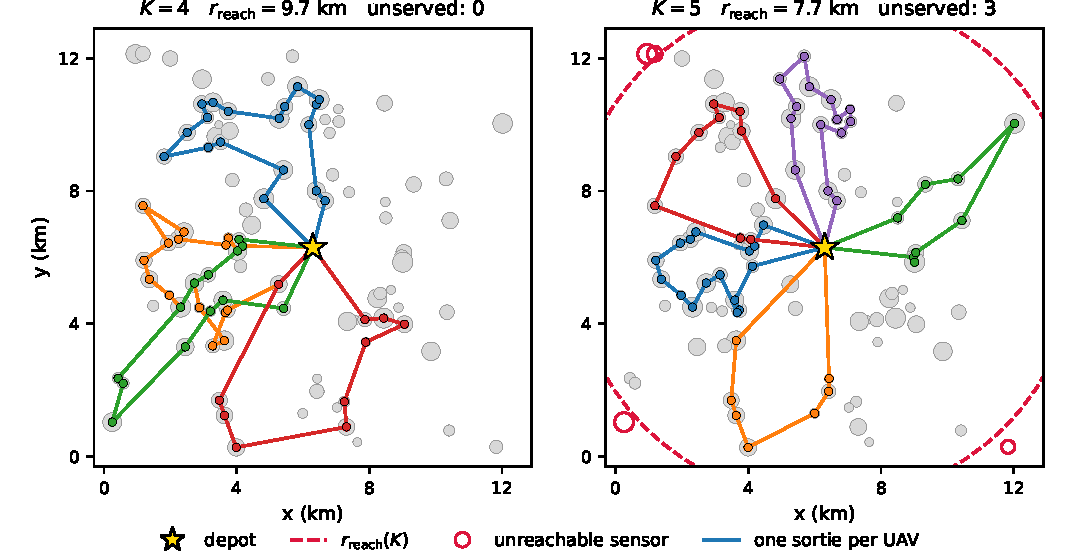
\includegraphics[width=.82\linewidth]{figs/fig1_reach}
\caption{The reach mechanism. One sortie per UAV on the same instance ($M=100$, $\Emax=1.5$~MJ, hour 6), at the fleet size given by the rule ($K=4$) and one UAV beyond it ($K=5$). Marker area scales with sensor priority; the dashed circle is $r_{\mathrm{reach}}(K)$. Splitting the same battery across five UAVs shrinks the reachable set inside the field: four sensors in three corners fall outside it, and the three of them that are never served (red) age for the rest of the deployment. The objective rises from $J=8.02\times10^{5}$ to $1.16\times10^{6}$ (seed 1).}
\label{fig:teaser}
\end{figure*}

Section~\ref{sec:model} states the model. Section~\ref{sec:law} derives the rule. Section~\ref{sec:planner} describes the planner and the coordination mechanism. Section~\ref{sec:eval} validates the rule and its exceptions on 3{,}801 simulation runs across 272 deployments and reports the information-value experiment. Section~\ref{sec:disc} discusses limitations, and Section~\ref{sec:conc} concludes.

\section{Related Work}\label{sec:related}

\textit{Which freshness metric.} Age of information is conventionally a receiver-side quantity: the age of the newest update at the monitor \cite{yates2021aoi}. We study \emph{age at collection}, the time since a UAV last drained a sensor, which Proposition~\ref{prop:buffer} makes exactly $t-t^{\mathrm{last}}$. This coincides with AoI wherever the collecting UAV is itself the consumer of the updates, as in multi-UAV data collection that measures AoI at the UAVs \cite{wang2023cooperative} and DRL formulations that minimise the weighted AoI of processes at the UAV \cite{abdelmagid2019drl}. It is also the age, or idleness, of the persistent-surveillance and patrolling literature, where a cell's age is the time since it was last observed \cite{nigam2014review}. It differs from sink-side formulations whose AoI also includes flight and offloading time after collection \cite{gao2023aoi}; results stated for one metric should not be read as claims about the other.

\textit{AoI scheduling.} For a single server with unreliable channels, randomized, Max-Weight and Whittle-index scheduling policies come with performance guarantees, and the latter two are near-optimal in simulation \cite{kadota2018scheduling}, and the Whittle-index policy is proved optimal for two sources with reliable channels and suggested to be close to optimal in general \cite{tripathi2019whittle}. Our planner's index is related to these but distinct: it is linear in age ($w\hat a/e$) where theirs are quadratic, and it selects an energy-constrained set; Section~\ref{sec:eval} shows why this suffices.

\textit{UAV data collection for AoI.} UAV-assisted data collection is surveyed in \cite{wei2022survey,mozaffari2019tutorial}, and AoI minimisation in UAV-aided collection is reviewed systematically in \cite{amodu2023review}. Trajectory design has been treated by joint optimisation of trajectory and resource allocation for a UAV relay \cite{abdelmagid2019peak}, by DRL \cite{abdelmagid2019drl}, and for multiple UAVs with peak- and average-AoI objectives, the number of UAVs following from endurance feasibility \cite{gao2023aoi}; the first two take the fleet as given. Liu et al.\ \cite{liu2022aoi} assign sensors and order tours jointly for a fixed number of UAVs with a multi-population genetic algorithm.

\textit{Fleet size.} Choosing how many vehicles to operate, jointly with their routes, is classical in operations research: the fleet size and mix vehicle routing problem trades fixed vehicle costs against routing costs \cite{golden1984fsm}, and fleet composition and heterogeneous routing are surveyed in \cite{hoff2010fleet,koc2016thirty}. There the vehicles are independent, each with its own capacity, so adding one never shortens another's route; the trade-off is cost against service, not the division of a shared resource. Prior work has also treated UAV count in several freshness-related formulations. Multi-UAV AoI studies have observed an interior optimum in the number of UAVs, caused by interference among independently powered UAVs \cite{wang2023cooperative}; others select the minimum number of UAVs for an AoI objective by mixed-integer programming \cite{tekin2025secure}, or minimise the number of UAVs needed to meet battery and data-age constraints \cite{yu2025fleet}; with collection by hovering over each sensor, the route construction of \cite{yu2025fleet} is the shortest nearest-neighbour tour over all start nodes, cut into segments that meet both the energy and the data-age constraint, followed by a rebalancing step that paper does not specify in full. Our tour patrol is close to this construction: it starts the nearest-neighbour tour at the depot, improves it by 2-opt, has no deadline and flies the tour cyclically. In persistent monitoring, the minimum number of robots meeting revisit-latency constraints with recharging has been bounded by approximation algorithms \cite{asghar2025persistent}, and single-UAV patrols have been optimised for time-average AoI \cite{wangxu2025patrol}. These treat fleet size through numerical optimisation, through feasibility constraints on independently powered agents, or both; with independent batteries, adding an agent never shortens another's range. We have not found work that derives a design-time rule for the AoI-optimal airborne fleet size under a fixed fleet-level energy inventory, in which each additional UAV adds parallelism and reduces the energy of every sortie, or that identifies the reach and commute regimes studied here. The interference optimum of \cite{wang2023cooperative} is the case Remark~\ref{rem:budget} anticipates: a finite optimum under independent batteries requires a different shared bottleneck, there spectrum.

\textit{Learned policies.} Learned combinatorial optimisation is surveyed in \cite{bengio2021mlco}, and attention-based policies have been trained for routing problems \cite{kool2019attention}. For UAV data collection with an AoI objective, multi-agent DRL has been applied to threshold-AoI crowdsensing \cite{wang2024drlucs}; Section~\ref{sec:eval:baseline} reports our attempt to reproduce it. Section~\ref{sec:eval:info} bounds one channel through which a learned policy could gain here --- explicit event-state information --- not every channel, and Section~\ref{sec:eval:baseline} tests the fleet-size optimum under independent planners.

\section{System Model}\label{sec:model}
Table~\ref{tab:notation} collects the notation.

\begin{table}[t]\centering
\footnotesize\setlength{\tabcolsep}{3pt}
\caption{Notation.}
\label{tab:notation}
\resizebox{\columnwidth}{!}{%
\begin{tabular}{ll}
\toprule
$M$, $K$ & sensors, UAVs\\
$L$ & field side; depot at the centre\\
$r_i$, $\rmax$ & sensor radius from depot; largest of them\\
$\rc$ & realised commute radius (depot to first/last stop)\\
$\Emax$, $\rho$, $U$ & energy inventory, reserve fraction, usable $U=(1-\rho)\Emax$\\
$\Eu$ & per-sortie budget $U/K$\\
$v$, $\Pf$, $\Ph$, $\Pbar$ & speed, flight/hover/mean productive power\\
$\Ru$, $B$, $\lambda_i$ & uplink rate, buffer size, generation rate\\
$w_i$, $g$ & sensor priority; event-age coefficient\\
$\tilde A_i$ & informational age of sensor $i$ (Prop.~\ref{prop:buffer})\\
$t_c$, $n$, $T_s$, $\tau_s$ & commute time, stops, sortie time, time per stop\\
$\Kr$, $K_{\mathrm{flight}}$ & full-buffer and flight-only reach caps\\
$\Kc$ & commute cap\\
$\mathcal{P}(t)$ & fleet route commitments with ETAs\\
$b_i$, $q$, $\bar\tau$ & event belief, event correlation, event lifetime\\
\bottomrule
\end{tabular}%
}
\end{table}

\subsection{Field, fleet and energy}
$M$ sensors sit at fixed positions $x_i$ in a square field of side $L$ with a depot at the centre; $r_i=\|x_i-x_0\|$ is the distance of sensor $i$ from the depot and $\rmax=\max_i r_i$. Sensor $i$ has baseline priority $w_i>0$ and generates data at rate $\lambda_i$ into a buffer of capacity $B$ bits with drop-head overflow (oldest data discarded). A UAV serves a sensor by hovering over it and uploading its buffer at rate $\Ru$, taken constant: the UAV hovers directly above the sensor at fixed altitude, so the air-to-ground link is at its shortest range and near-certain line of sight for the whole of the upload. A range- or channel-dependent rate would replace the fixed $\Ru$ by an achievable rate at the hover point and therefore alter only the dwell time $t_d=\min(\lambda_i\tilde A_i,B)/\Ru$; both caps take $\Ru$ only through the cap-dwell term $\Ph B/\Ru$ in \eqref{eq:Kreach} and through $\tau_s$ in \eqref{eq:R}, so the structure of the rule is unchanged and its constants shift. We do not model inter-UAV interference: each UAV's uplink is assumed independent of the others'. The coordination rule of Sec.~\ref{sec:model:coord} prevents two UAVs from serving the same sensor but does not deconflict trajectories or radio links; uploads are short relative to sortie duration, which limits simultaneous transmission, but we do not claim that it removes interference. Sensor-side transmit energy and duty cycling are likewise outside the model; they would enter as an upper constraint on $t_d$, in the same place as the buffer cap, and therefore act on both branches exactly as $B/\Ru$ does.

The fleet has $K$ UAVs sharing a usable energy inventory $U=(1-\rho)\Emax$, where $\rho$ is a safety reserve, so each sortie has budget $\Eu=U/K$.

\begin{remark}[What the shared budget means, and when it applies]\label{rem:budget}
Every result below follows from $\Eu=U/K$, so the assumption deserves to be stated plainly. We are \emph{not} modelling $K$ independent airframes each carrying its own battery; there, per-sortie energy is a constant of the airframe, total energy is proportional to $K$, and no reach cap exists. We model the case in which the energy the fleet can carry aloft is fixed and adding airframes divides it: $K$ simultaneously airborne UAVs share an inventory $U$, so each carries $U/K$. This is the situation of a fixed total \emph{modular} battery capacity divided equally among the simultaneously airborne UAVs --- a configurable number of battery modules per airframe, with swapping and recharging fast enough not to bind --- or of fleets compared at equal total battery capacity --- equal battery mass or battery cost --- rather than equal per-airframe capability. Concretely: a field team deploys with a fixed pool of battery modules and airframes that accept a variable number of them; some modules fly while the rest recharge. Flying two airframes with four modules each or eight with one each is exactly the choice of $K$ at fixed $U$. Shared battery pools serving several UAVs through automated swap-and-recharge stations are established practice for persistent missions \cite{toksoz2011swap,suzuki2012battery}; what the model adds is the modular bay, which lets the airborne share of the pool be divided among however many airframes fly. Without it, a swap station gives every sortie a whole pack whatever $K$ is, which is the independent-battery case below. $U$ is a stock, not a rate: $\Emax$ is the total energy inventory, not a single battery, and each UAV's sortie is limited by its share of it. It is \emph{not} a model of a charging station of fixed power. With all $K$ UAVs airborne and instant turnaround, the fleet draws about $K\Pbar$ on average ($0.3$--$0.4$~kW per airborne UAV here), which grows with $K$; a charger of fixed power $P_c$ therefore imposes a different constraint, $K\Pbar\le P_c$, a cap on the airborne count that does not act through $\Eu$ and that we do not model. Where energy is not the shared resource---each airframe carrying its own fixed battery $\Eu=E_0$, with abundant charging and no other bottleneck---\emph{neither} cap yields a finite optimum. The reach radius no longer shrinks with $K$, so \eqref{eq:Kreach} does not bind; and since $n$ and $T_s$ are then $K$-independent, the fleet visit rate $\Gam\approx Kn_0/T_{s,0}$ (Section~\ref{sec:law:commute}; $n_0$ stops per sortie of duration $T_{s,0}$, both fixed by $E_0$) is monotone increasing, so the commute branch does not bind either. Commute overhead still makes each sortie less efficient, but it does not make an additional independently powered UAV harmful. The non-monotone fleet-sizing problem studied here therefore arises from a shared fleet-level resource; with independent per-airframe energy a finite optimum would require some other shared bottleneck --- charging throughput, spectrum, operator attention, or airspace congestion near the depot --- which we do not model.

An operator who owns more airframes than the inventory usefully supports could try to evade $\Eu=U/K$ by flying them in rotation: keep each airborne a fraction $\delta$ of the time, so that the inventory is shared among $K\delta$ airborne UAVs and each sortie carries $U/(K\delta)$. Proposition~\ref{prop:duty} shows this does not evade the cap; it relocates it to the number of UAVs \emph{simultaneously airborne}, which is the quantity the rule sizes. The assumption in Section~\ref{sec:model} that all $K$ UAVs are airborne at all times is therefore the normalisation $\delta=1$, not an independent restriction.


\emph{Battery mass.} Dividing the inventory among $K$ airframes also divides its mass: each carries $\Emax/K$ of battery (its usable share $U/K$ and its share of the reserve), so a smaller fleet flies heavier, and rotor power rises with take-off mass (hover power as $m^{3/2}$ by momentum theory). Because $K$ is fixed within a deployment, each airframe's mass is constant during it, and every per-$K$ result holds with $\Pf$ and $\Ph$ evaluated at that $K$'s load; the reach cap becomes the fixed point $K=vU/(2\Pf(\Emax/K)\rmax+v\Ph(\Emax/K)B/\Ru)$. This does not carry over to the closed form $\Kc$, which differentiates $\Gam(K)$ at constant power; with mass-dependent power the commute cap is the numerical maximiser of $\Gam$. The constants we use are therefore the powers at one reference load. To size the effect, take a $2.0$~kg airframe, $180$~Wh/kg packs, our $\Pf,\Ph$ at a $0.5$~kg pack, hover power $\propto m^{3/2}$ and flight power $\propto m^{\gamma}$ with $\gamma\in[0.5,1.5]$ (the exponent depends on how much of flight power is induced). At the reach cap the battery is $16$--$21\%$ of take-off mass, and the fixed point, unique in every instance, lies $0.5$--$1.9\%$ above the constant-power $\Kr$ (medians over the 240 primary instances for $\gamma=0.5$ and $1.5$), changing $\lfloor\Kr\rfloor$ in 12 to 53 of them. The rule is exact only if $\Pf$ and $\Ph$ are the powers of the airframe carrying the reach-cap load; specifying them at another load is an input error of the kind studied in Section~\ref{sec:eval:exante}, and here it moves $\lfloor\Kr\rfloor$ in at most about a fifth of instances. Simulating mass-dependent power ($\gamma=1$; $M=100$, all three layouts, both budgets, 72 instances) confirms the direction and shows that the effect is small where the reach cap binds. The measured optimum rises from a mean of $7.8$ to $8.7$ UAVs, moving in $46\%$ of instances, but on clustered fields in only $8\%$ (1.5~MJ) and $25\%$ (3~MJ) of them, and there the constant-power rule keeps its exact agreement ($0.92$ and $0.67$). Over all 72 instances the constant-power rule falls to exact agreement $0.38$ and within-one $0.83$ (median regret $3.8\%$), and the fixed-point rule recovers $0.43$ and $0.83$ ($1.7\%$); the gain is on the core layout (exact $0.42\to0.50$ at 1.5~MJ and $0.08\to0.33$ at 3~MJ). It does not help on the ring, consistent with the closed-form commute cap not carrying over; our numerical commute cap scales $\Pbar$ with flight power, an approximation we have not refined.
\end{remark}

\begin{proposition}[Duty cycling does not evade the reach cap]\label{prop:duty}
Let the energy inventory $U$ be shared among the UAVs airborne at any time, and let each of $K$ airframes be airborne a fraction $\delta\in(0,1]$ of the time, resting on the pad otherwise, so that a sortie carries $\Eu=U/(K\delta)$. Write $K_{\mathrm{air}}=K\delta$ for the expected number of UAVs airborne. Then
\begin{enumerate}[label=(\roman*)]
\item every sensor can be served from any state iff $K_{\mathrm{air}}\le\Kr$, and some sensor is unreachable iff $K_{\mathrm{air}}>K_{\mathrm{flight}}$, with both caps exactly as in Section~\ref{sec:law:reach};
\item the fleet visit rate is $\Gam=K_{\mathrm{air}}n/T_s$ with $n$ evaluated at $\Eu=U/K_{\mathrm{air}}$, i.e.\ \eqref{eq:R} with $K$ replaced by $K_{\mathrm{air}}$;
\item consequently reachability and the aggregate visit-rate model depend on $(K,\delta)$ only through $K_{\mathrm{air}}$; under stationary, well-staggered duty cycling with $K$-invariant visit-interval statistics the same holds for the long-run objective $J$, and the rule of Result~\ref{thm:law} sizes $K_{\mathrm{air}}$.
\end{enumerate}
\end{proposition}
\begin{proof}
Substituting $\Eu=U/(K\delta)$ into \eqref{eq:rreach} gives $r_{\mathrm{reach}}=v(U/K_{\mathrm{air}}-\Ph B/\Ru)/(2\Pf)$, and requiring $\rmax\le r_{\mathrm{reach}}$ gives the first half of (i); the same substitution in $K_{\mathrm{flight}}=vU/(2\Pf\rmax)$ gives the second. A UAV completes a sortie every $T_s/\delta$ on average and serves $n$ sensors per sortie, so the fleet rate is $K\delta n/T_s$, giving (ii). The guaranteed and impossible sets, and the aggregate visit-rate model, then depend on $(K,\delta)$ only through $K_{\mathrm{air}}$; service of the intermediate gray set additionally depends on the scheduling policy. The served-set cost additionally depends on the inter-visit variability $(1+\mathrm{CV}_i^2)$ and, with events, on when UAVs are airborne rather than only how many; the stated staggering condition is what makes these invariant, giving (iii). The physical conclusion---that duty cycling does not evade the resource trade-off---does not need the stronger exact statement.
\end{proof}

Three qualifications. First, the airframe bounds the share: a sortie cannot carry more than the battery capacity $E_{\mathrm{batt}}$, so $U/K_{\mathrm{air}}\le E_{\mathrm{batt}}$, i.e.\ $K_{\mathrm{air}}\ge U/E_{\mathrm{batt}}$. The physical battery therefore enters the model as a \emph{floor} on the airborne fleet, complementary to the reach cap from above. Second, $K\delta$ need not be an integer; the equivalence holds in expectation, with the airborne count fluctuating around it and the coordination protocol seeing a varying fleet. Third, this is a small gain for the rule: since the airborne fleet is continuous, an operator can sit at $K_{\mathrm{air}}=\Kr$ exactly rather than at $\lfloor\Kr\rfloor$.

The practical reading is that buying more airframes and flying fewer of them at once buys nothing and costs nothing for freshness: it is the same fleet in the air. An operator with $K$ airframes should fly $\min(K,K^\star)$ of them continuously and leave the remainder as spares. This also disposes of the objection that a fifth UAV should not reduce the energy available to the first four---it does not, if the fifth is left on the ground.

\begin{remark}[Equal allocation]\label{rem:equal}
We allocate $U$ equally. This is not assumed optimal: with heterogeneous allocation the operator could fund one long-range sortie for a peripheral sensor and divide the remainder, which removes the abandonment that drives the reach branch. Equal allocation is the simplest symmetric policy for identical airframes drawing on one shared inventory. The gap matters most exactly where our reach branch is weakest: the \emph{core} family (one peripheral outlier, all other sensors near the depot) is the case in which a single long sortie dominates, and is also the family in which criterion~\eqref{eq:window_apriori} flags (Sec.~\ref{sec:eval:fail}). We regard heterogeneous energy allocation as the natural next question rather than a defect of the present model. Section~\ref{sec:eval:fail} tests the simplest case --- one UAV's energy share sized for the outlier's full-buffer out-and-back, the rest shared equally --- and, in the two cells tested, finds that it removes the stranding regime and restores the reach mechanism for the remaining UAVs.
\end{remark} A UAV flies at speed $v$ with flight power $\Pf$ and hovers with power $\Ph$; flying distance $d$ costs $\Pf d/v$ and hovering for $t$ costs $\Ph t$. For a rotary-wing airframe propulsion power is a function $P(V)$ of airspeed \cite{zeng2019energy}; at a fixed cruise speed it is the constant $\Pf=P(v)$, and $\Ph=P(0)$, which exceeds $\Pf$ at moderate speeds. A sortie starts and ends at the depot, must respect $\Eu$ including the return leg, and a UAV relaunches immediately on landing, except after a sortie that served nothing: it then waits $t_c$ (about 8~min here) on the pad before planning again. Such empty sorties are rare at the optimum (median $0\%$ of sorties; at most $1.6\%$ on clustered fields, $9.3\%$ on the core layout and $0.8\%$ on the ring). The rule is enforced twice. Before each leg, the UAV checks that it can fly to the next stop and from there to the depot; if not, it flies home. On arrival, if serving the stop with its realised dwell and then returning would exceed the remaining energy, the stop is not served and the UAV flies home from it. The reserve $\rho\Emax$ is therefore never used. All $K$ UAVs are airborne at all times except during these waits; turnaround is otherwise instantaneous.

\subsection{Events}
Sensors experience \emph{events}: transient periods during which their data is urgent. Events fire as a Poisson process with rate $\nu_i$ ($\nu_{\mathrm{hot}}$ for sensors inside hotspots, $\nu_{\mathrm{cold}}$ otherwise), last a random duration $\tau\sim\mathcal{U}(\tau_{\mathrm{lo}},\tau_{\mathrm{hi}})$, and are cleared by a visit. A firing at a sensor whose event is still live extends that event to the later of the two end times and keeps its original fire time, so event age counts from the first uncaught firing; the live periods of a sensor are then the busy periods of an M/G/$\infty$ queue, and, absent visits, a sensor is live with stationary probability $1-e^{-\nu_i\bar\tau}$, $\bar\tau=\mathbb{E}[\tau]$. An uncaught episode lasts $(e^{\nu_i\bar\tau}-1)/\nu_i$ on average: $2.1$~h for a hotspot sensor and $74$~min elsewhere at the parameters of Section~\ref{sec:eval:setup}, against $\bar\tau=67.5$~min for a single event. A UAV observes a sensor's event state only on arrival. In Section~\ref{sec:eval:info} we additionally let events be spatially correlated: a hotspot fires as a unit at rate $\nu_{\mathrm{hot}}/q$ and each member goes live with probability $q$, so each member's event rate stays $\nu_{\mathrm{hot}}$ and $q$ changes only the correlation ($q=0$ means independent events).

\subsection{Objective}
Let $\tilde A_i(t)$ be the informational age of sensor $i$ (Proposition~\ref{prop:buffer}), equal to the time since its last visit, $t-t^{\mathrm{last}}_i$, and let $t^{f}_i$ be the fire time of a live, uncaught event at $i$. The fleet minimises
\begin{equation}\label{eq:J}
J=\frac{1}{T}\int_{T_b}^{T_b+T}\Big[\sum_{i=1}^{M} w_i\tilde A_i(t)+\sum_{i\in\mathcal{E}(t)} g\,w_i\,(t-t^{f}_i)\Big]dt,
\end{equation}
where $\mathcal{E}(t)$ is the set of sensors with a live uncaught event, $g$ prices event age relative to baseline priority, $T_b$ is a burn-in, and $T$ the measurement window. The first term is priority-weighted buffer age; the second is event AoI. We refer to them as $J_{\mathrm{age}}$ and $J_{\mathrm{event}}$.

\begin{remark}
An earlier formulation multiplied $w_i$ by $g$ while an event was live, charging the entire buffer backlog as urgent the instant an event fired. That rewards visiting stale sensors that happen to have events rather than catching events quickly. Equation~\eqref{eq:J} charges the event's own age.
\end{remark}

\subsection{Fleet state and coordination}\label{sec:model:coord}
At any time the fleet state is $(\tilde A(t),\mathcal{P}(t))$, where $\mathcal{P}(t)=\{(j,\hat t_j)\}$ is the set of sensors committed in the routes of currently airborne UAVs with estimated arrival times. A UAV that plans at time $t$ excludes from its candidate set every sensor that appears in the remaining route of any other airborne UAV, regardless of which would arrive first; commitments are reported to the depot at launch and at every replan, the depot recomputes their estimated arrival times from the committing UAVs' current positions, and every planner sees the latest state. No inter-UAV link is assumed beyond the depot. Because a committed sensor is excluded from every other planner's candidate set, commitments are not pre-emptible: the first UAV to claim a sensor keeps it, so no UAV can have its target taken while in transit. Section~\ref{sec:eval:replan} tests whether allowing UAVs to abandon a leg in response to later state changes pays. Section~\ref{sec:eval:coord} quantifies what happens without this.

\subsection{Decision structure}
A UAV decides its route at launch and, optionally, re-optimises its remaining route after every stop from its current position and remaining energy (\emph{per-leg replanning}). Both variants are evaluated. Any routing policy---optimiser or learned---operates within this structure with the same information, which is what makes the comparison in Section~\ref{sec:eval:info} fair.

\section{Buffer Cancellation}\label{sec:buffer}
\begin{proposition}[Buffer cancellation]\label{prop:buffer}
Under drop-head overflow and full drainage at each visit, define the informational age of sensor $i$ as the age of its oldest retained sample plus the time span covered by samples destroyed by overflow since the last visit. Then $\tilde A_i(t)=t-t^{\mathrm{last}}_i$ for any generation-rate process with $\lambda_i>0$ after $t^{\mathrm{last}}_i$, and the buffer capacity $B$ enters the objective~\eqref{eq:J} only through the dwell-time cap $t_d\le B/\Ru$.
\end{proposition}
\begin{proof}
After a full drain at $t^{\mathrm{last}}_i$ the buffer refills. Before saturation the oldest retained sample was generated at $t^{\mathrm{last}}_i$, so its age is $t-t^{\mathrm{last}}_i$ and nothing has been destroyed. After saturation, the oldest retained sample has age $a(t)$, where $\int_{t-a(t)}^{t}\lambda_i(s)\,ds=B$ (the buffer holds exactly the most recent $a(t)$ seconds of data in a fluid model; $a=B/\lambda_i$ for a constant rate), and the destroyed samples cover the span $[t^{\mathrm{last}}_i,\,t-a(t)]$ of length $t-a(t)-t^{\mathrm{last}}_i$. The sum is $t-t^{\mathrm{last}}_i$ in both cases. Defining the destroyed charge as a time span rather than a bit count makes the identity independent of $\lambda_i(t)$. The only place $B$ survives is the upload time at a visit, $\min(\lambda_i\tilde A_i, B)/\Ru$.
\end{proof}

The proposition is an identity that follows from the definition of informational age; its content is the choice of that definition, which charges lost data by the time span it covered rather than by its volume, and its use is that buffer capacity then leaves the objective. Two consequences matter for what follows. Age is reset at collection, not at delivery to the depot; this is the ``age at collection'' convention of Section~\ref{sec:intro} and is stated as such. And partial drainage would break the identity, so the planner never partially serves a sensor: if the remaining energy cannot cover a full service plus the return leg, the sensor is not served and the UAV abandons the rest of its route and flies home.

\section{The Fleet-Sizing Rule}\label{sec:law}

\subsection{Reach branch}\label{sec:law:reach}
Any sortie that serves sensor $i$ must fly at least $r_i$ from the depot to reach it and at least $r_i$ back (triangle inequality), and the direct out-and-back sortie attains this minimum, so $2\Pf r_i/v+\Ph t_{d,i}$ is the least energy with which $i$ can be served. The dwell $t_{d,i}=\min(\lambda_i\tilde A_i,B)/\Ru$ depends on how long $i$ has waited, which gives two bounds rather than one. A sensor with a \emph{full} buffer can be served iff
\begin{equation}\label{eq:rreach}
r_i\le r_{\mathrm{reach}}(K)=\frac{v\,(U/K-\Ph B/\Ru)}{2\Pf},
\end{equation}
so every sensor can be served from any state iff
\begin{equation}\label{eq:Kreach}
K\le\Kr\equiv\frac{vU}{2\Pf\rmax+v\Ph B/\Ru}.
\end{equation}
With no dwell at all the farthest sensor is out of reach iff $K>K_{\mathrm{flight}}\equiv vU/(2\Pf\rmax)$, which is therefore the exact upper limit. Between the two the farthest sensors remain serviceable only while they are revisited before their backlog exceeds $b^{\star}_i(K)=\Ru(U/K-2\Pf r_i/v)/\Ph<B$, the largest backlog a direct out-and-back can still upload. Backlog only grows between visits, so such a sensor is lost once its gap between visits exceeds $b^{\star}_i(K)/\lambda_i$. The bracket is narrow --- $K_{\mathrm{flight}}/\Kr=1+v\Ph B/(2\Pf\rmax\Ru)$, between $1.025$ and $1.072$ here --- but it contains an integer in 119 of 272 instances, and our planners do sustain such schedules: at paper $M=50$, 3~MJ, $K=11$ ($\Kr=10.77$, $K_{\mathrm{flight}}=11.28$) the two sensors beyond the full-buffer radius are each visited 40--47 times after burn-in, with their buffers never more than $16\%$ full. We use the full-buffer cap $\Kr$ --- the \emph{robust} reach cap, which guarantees service from any state without assuming a revisit schedule --- as the reach branch of the rule. Substituting $K_{\mathrm{flight}}$ raises exact agreement over all 272 instances from $0.56$ to $0.67$ ($0.55$ to $0.65$ over the 240 primary instances) with within-one agreement unchanged (Sec.~\ref{sec:eval:law}), which shows that part of the rule's small positive bias in reach-bound fields (measured optimum above the rule) is this bracket rather than any error in the mechanism. We nevertheless keep $\Kr$, because the gain from operating inside the bracket is bought with a failure mode the steady-state grid cannot show: a gray-set sensor is lost permanently as soon as its backlog exceeds $b^{\star}_i(K)$, so a single service interruption longer than $b^{\star}_i(K)/\lambda_i$ removes it for the rest of the deployment. Section~\ref{sec:eval:law} quantifies the trade-off and gives the condition under which the flight-only cap is the better choice.
For $K>K_{\mathrm{flight}}$ at least one sensor is never served, and for $\Kr<K\le K_{\mathrm{flight}}$ one is lost as soon as its backlog is allowed to exceed $b^{\star}_i(K)$. Formally, at fleet size $K$ the sensors split into three sets: $\mathcal{S}_{\mathrm{guar}}(K)=\{i:2\Pf r_i/v+\Ph B/\Ru\le U/K\}=\{i:r_i\le r_{\mathrm{reach}}(K)\}$, serviceable from any buffer state; $\mathcal{A}_{\mathrm{imp}}(K)=\{i:2\Pf r_i/v>U/K\}$, which no schedule can serve; and the schedule-dependent \emph{gray set} $\mathcal{G}(K)$ of the remainder, served only while a planner keeps their backlog below $b^{\star}_i(K)$. A sensor that is never visited contributes $C_i(T)=w_i(T_b+T/2)$ to the age term of \eqref{eq:J} (its uncaught events add further event age, which $C_i$ leaves out); $C_i$ grows linearly with the window and diverges as $T\to\infty$; for finite $T$ it is a finite cost that can rationally be traded against better service to the rest of the field, which is what the core family does. Writing $J(K)=J_s(K)+\sum_{i\in\mathcal{A}(K)}C_i(T)$ with $J_s$ the served-set cost and $\mathcal{A}(K)$ the abandoned set, we have:

\begin{lemma}[Finite-window condition, one step]\label{lem:window}
If $\mathcal{A}(\lfloor\Kr\rfloor)=\emptyset$ and the sensors of $\mathcal{A}(\lfloor\Kr\rfloor+1)$ are never visited, then $J(\lfloor\Kr\rfloor)<J(\lfloor\Kr\rfloor+1)$ whenever
\begin{equation}\label{eq:window}
\begin{aligned}
&(T_b+T/2)\sum_{i\in\mathcal{A}(\lfloor\Kr\rfloor+1)}w_i\\
&\qquad>J_s(\lfloor\Kr\rfloor)-J_s(\lfloor\Kr\rfloor+1),
\end{aligned}
\end{equation}
\end{lemma}
This is a \emph{local} crossing condition: it rules out $\lfloor\Kr\rfloor+1$, not every larger fleet. A fleet can be worse at one more UAV and better at five more, which is exactly what the core family does. The global statement $K^{\star}=\lfloor\Kr\rfloor$ follows if, in addition, $J(K)\ge J(\lfloor\Kr\rfloor+1)$ for all $K>\lfloor\Kr\rfloor+1$ and $J(K)>J(\lfloor\Kr\rfloor)$ for $K<\lfloor\Kr\rfloor$, or from a one-crossing property we have not proved. Without the lemma's first condition the step changes by $\sum_{\mathcal{A}(\lfloor\Kr\rfloor+1)}C_i-\sum_{\mathcal{A}(\lfloor\Kr\rfloor)}C_i$ instead, and $\lfloor\Kr\rfloor\le\Kr$ means only that every sensor \emph{can} be served, not that it is: at clustered $M=400$, 1.5~MJ, 1--7 in-reach sensors go unserved at $\lfloor\Kr\rfloor$ in 10 of 12 seeds. The design-time criterion~\eqref{eq:window_apriori} below is the global form we actually use: it compares the surrogate objective at $\lfloor\Kr\rfloor$ with every larger fleet rather than one step.
The left side grows with the window; the right side does not. As stated, \eqref{eq:window} requires $J_s$ at two fleet sizes and so is not checkable before running the system, and it compares against only the next fleet size, whereas an operator who abandons a sensor may keep adding UAVs as long as the served set keeps improving. The design-time form therefore evaluates the surrogate objective of Proposition~\ref{prop:sqrt} at every larger fleet size instead of one step. With the radial cost surrogate $c_i^{\mathrm{rad}}=2\Pf r_i/v$ and $C(K)=\Pbar\,\Phi(K)$ ($\Phi$ is the visit-rate factor defined after \eqref{eq:R} below), write
\[
\begin{aligned}
F(K)&=\frac{Q_K^2}{2C(K)}+(T_b+T/2)\!\!\sum_{i\notin\mathcal{S}_{\mathrm{guar}}(K)}\!\!w_i,\\
Q_K&=\sum_{i\in\mathcal{S}_{\mathrm{guar}}(K)}\sqrt{w_ic_i^{\mathrm{rad}}},
\end{aligned}
\]
the served-set freshness at the ideal allocation plus the age cost of every sensor without a full-buffer guarantee. The criterion is
\begin{equation}\label{eq:window_apriori}
\begin{gathered}
F(K)>F(\lfloor\Kr\rfloor)\\
\text{for every integer }K\in\big(\lfloor\Kr\rfloor,\,K_{\max}\big],
\end{gathered}
\end{equation}
where $K_{\max}$ is the largest fleet with $\Phi(K)>0$. It asks whether $\lfloor\Kr\rfloor$ minimises the surrogate over all larger fleets, so it is exact within the surrogate and needs no one-crossing property; the served set is allowed to shrink with $K$, as it must. Every quantity follows from the sensor set, the airframe, the commute inputs $(\rc,\Pbar)$ and the operating window, and evaluating it takes a closed-form expression at a few dozen to a few hundred integers. Its error relative to the realised objective is the surrogate's, not a bounding error, and it has four parts with known directions. First, the abandoned set is the full-buffer one, which charges gray-set sensors as abandoned although a planner may keep them serviceable and so pushes the verdict toward passing. This is not confined to the reach bracket, because at every larger $K$ other sensors fall into $\mathcal{G}(K)$: the charge changes 31 of the 168 verdicts, all toward passing, including that of the largest passing regret. Second, the abandoned cost counts only the age term; a never-visited sensor also accrues uncaught event age ($+66\%$ for a hotspot sensor and $+7\%$ elsewhere over the $12$~h horizon), and leaving it out errs toward flagging. Third, the commute inputs are held at their smallest-$K$ values; using $\rc(K)$ and $\Pbar(K)$ changes 9 of 168 verdicts, 8 of them toward passing, so fixed inputs also err toward flagging. Fourth, the served-set term prices every visit at $c_i^{\mathrm{rad}}$, the energy of a dedicated out-and-back flight, which overstates the energy a visit costs inside a multi-stop sortie; the next lemma shows that this choice of scale errs toward flagging.

\begin{lemma}[Cost scale]\label{lem:scale}
Let the served-set term use $c_i=\kappa c_i^{\mathrm{rad}}$ for a constant $\kappa\in(0,1]$, and write $F_\kappa$ for the resulting $F$ and $\hat K_\kappa$ for the stopping point of Proposition~\ref{prop:strand} (Section~\ref{sec:eval:fail}). (i) If \eqref{eq:window_apriori} holds for $F_1$, it holds for $F_\kappa$. (ii) $\hat K_\kappa$ is non-decreasing in $\kappa$.
\end{lemma}
\begin{proof}
For $K>K_0=\lfloor\Kr\rfloor$ write $F_\kappa(K)-F_\kappa(K_0)=\kappa\,\Delta_s(K)+\Delta_a(K)$, with $\Delta_s$ the change in the served-set term $Q_K^2/2C(K)$ at $\kappa=1$ and $\Delta_a$ the change in the abandoned term. Since $r_{\mathrm{reach}}(K)$ decreases in $K$, $\mathcal{S}_{\mathrm{guar}}(K)\subseteq\mathcal{S}_{\mathrm{guar}}(K_0)$ and $\Delta_a(K)\ge0$, so $\kappa\Delta_s+\Delta_a\ge\kappa(\Delta_s+\Delta_a)$, which is positive whenever $F_1(K)>F_1(K_0)$; this is (i). Condition \eqref{eq:strand} at scale $\kappa$ reads $\kappa\,\mathrm{gain}(K)>\mathrm{loss}(K)$, with $\mathrm{gain}(K)$ its left side at $\kappa=1$ and $\mathrm{loss}(K)\ge0$ its right side; if it holds at $\kappa$ it holds at every $\kappa'>\kappa$, so the first failure cannot come earlier, which is (ii).
\end{proof}
The scale that matches the energy a stop actually costs is $\kappa=\Pbar\tau_s v/(2\Pf\bar r)$, with $\bar r$ the mean sensor distance from the depot, which sets the mean visit cost to the measured energy per stop; it is a median $0.18$ (range $0.11$--$0.48$) over our reach-bound instances. By the lemma the radial scale is the conservative choice for the criterion: in the 168 reach-bound instances no verdict that passes at $c_i^{\mathrm{rad}}$ fails at the measured scale, while 56 that it flags would pass there, 24 of them core instances with regret up to $34\%$ (10 above $10\%$). We therefore keep $c_i^{\mathrm{rad}}$, which needs no measurement, in the criterion. Sufficient-type variants that pair the smallest abandoned set with the largest served gain over all larger fleets are also valid within the surrogate, but they flag $88\%$ and $94\%$ of the clustered instances in which the rule loses nothing, so we do not use them. The criterion is design-time in the sense that no fleet sweep or simulation is needed, but it takes the commute inputs $(\rc,\Pbar)$, which are measured in this paper; Section~\ref{sec:eval:exante} shows that estimating them before deployment, at the smallest candidate fleet size, changes 3 of 168 verdicts and neither of the properties we report. Section~\ref{sec:eval:regret} evaluates it on every instance, and Table~\ref{tab:horizon} shows how the objective changes between a 12-hour and a 24-hour horizon.

\subsection{Commute branch}\label{sec:law:commute}
Below the robust reach cap every sensor is serviceable from any state, and the objective is governed by how often sensors are served. Model a sortie as an out-and-back commute of duration $t_c=2\rc/v$, where $\rc$ is the \emph{realised} commute radius (distance from the depot to the first and last served sensors), followed by $n$ productive stops each of duration $\tau_s$ at mean productive power $\Pbar$, a time-weighted average of hop and hover power (measured 301--400~W here). Then $n=(\Eu-\Pf t_c)/(\Pbar\tau_s)$, $T_s=t_c+n\tau_s$, and the fleet visit rate is
\begin{equation}\label{eq:R}
\Gam(K)=\frac{Kn}{T_s}=\frac{1}{\tau_s}\cdot\frac{K\,(U-K\Pf t_c)}{U+K t_c(\Pbar-\Pf)}.
\end{equation}
If served-sensor age is proportional to $1/\Gam$ (equal weights, no inspection-paradox correction), then $\arg\min_K J_s=\arg\max_K \Gam$, and setting $d\Gam/dK=0$ gives (Appendix~\ref{app:commute})
\begin{equation}\label{eq:Kcommute}
\Kc=\frac{U}{t_c\,(\Pf+\sqrt{\Pf\Pbar})}=\frac{vU}{2\rc\,(\Pf+\sqrt{\Pf\Pbar})}.
\end{equation}
Before listing the approximations, one apparent one can be removed outright. The sortie duration
\[
T_s=t_c+n\tau_s=t_c+\frac{\Eu-\Pf t_c}{\Pbar}
\]
does not contain $\tau_s$: the product $n\tau_s$ is fixed by the energy left after commuting, so how that energy is split between many short stops and few long ones changes $n$ and $\tau_s$ in compensating ways but not the length of the flight. Writing $\Phi(K)=\tau_s\Gam(K)=K(U-K\Pf t_c)/(U+Kt_c(\Pbar-\Pf))$, we have $\Gam=\Phi/\tau_s$ exactly.

\begin{proposition}[Backlog-dependent dwell does not move the optimum]\label{prop:tau}
In steady state with no buffer overflow the fleet must collect exactly what the field generates, so the fleet's total hovering time per unit time is $H=\sum_i\lambda_i/\Ru$, \emph{independent of $K$}. Consequently the dwell component of a stop is $H/\Gam(K)$, giving $\tau_s=\tau_{\mathrm{hop}}+H/\Gam(K)$, and therefore
\[
\Gam\,\tau_s=\Gam\,\tau_{\mathrm{hop}}+H=\Phi(K)\quad\Longrightarrow\quad \Gam(K)=\frac{\Phi(K)-H}{\tau_{\mathrm{hop}}} .
\]
Hence the \emph{dwell} component cancels exactly, and
\[
\arg\max_K\Gam(K)=\arg\max_K\frac{\Phi(K)-H}{\tau_{\mathrm{hop}}(K)},
\]
which reduces to $\arg\max_K\Phi$ if the inter-stop travel time $\tau_{\mathrm{hop}}$ is itself $K$-invariant.
\end{proposition}
This is worth stating because dwell \emph{does} vary with $K$ --- larger fleets visit more often, find smaller backlogs and dwell for less time --- and one would expect that to matter. It does not: the conservation law makes it cancel identically. The no-overflow condition is what makes the conservation law applicable, and it holds where we use it: on the ring at 3~MJ ($M=100$, $K=4,6,8$, two seeds) no served visit finds a full buffer and no data are dropped, and at 1.5~MJ the fraction of generated data dropped is $0.12\%$ at the optimum $K=3$ and at most $1.6\%$ in any run over $K=2$--$4$. Overflow becomes material only once sensors are stranded ($66\%$ of generated data lost at $K=6$, where 66 of 100 sensors are never served on average), outside the regime in which the proposition is invoked. The cancellation is exact for a given $\Phi(K)$, which takes $\Pbar$ as fixed; dwell does reach the optimum through $\Pbar$, the time-weighted mix of hover and flight power, but only weakly: per instance, $\Pbar$ varies by a median $1.1$--$1.4\%$ across stranding-free fleet sizes in the three families (at most $6.8\%$).

The hop component is a different matter, and we do not assume it away. Measuring travel time per stop directly, $\tau_{\mathrm{hop}}$ falls by $2$--$27\%$ over the swept range of the clustered cells ($51.5\to48.9$~s from $K=2$ to $4$ at $M=100$, 1.5~MJ) and by $21$--$65\%$ on the ring ($42.5\to26.2$~s from $K=4$ to $8$ at $M=100$, 3~MJ), because smaller budgets select tighter groups of stops. The ring is precisely where the commute branch binds, so this is not a negligible correction there --- and following it through resolves the discrepancy reported in Section~\ref{sec:eval:fail}. Substituting each instance's measured $\tau_{\mathrm{hop}}(K)$ into Proposition~\ref{prop:tau} moves $\arg\max\Gam$ from $6$, where $\Phi$ alone peaks, to a mean of $8.00$ against a measured mean $\arg\min J$ of $7.92$, within one UAV of it in all 12 instances against 1 of 12 for $\Phi$ alone; on the other two 3~MJ ring cells it gives $8.83$ against $8.50$ ($M=50$; within one in 10 of 12, against none for $\Phi$) and $7.00$ against $6.67$ ($M=200$). The closed form's error in the ring family is therefore attributable to a single measurable quantity, with no fitted exponent involved. Nor is the decline a property of our planner: an age-blind route-first patrol shows the same effect on the ring, $\tau_{\mathrm{hop}}$ falling from $32.8$ to $22.8$~s between $K=4$ and $8$ against $42.5$ to $26.2$~s for the annealer on the same cell. The conservation law also yields a throughput bound in its own right: the fleet pays a fixed hovering power $\Ph\sum_i\lambda_i/\Ru$ whatever its size, so a deployment whose generation rate exceeds what the energy budget can drain is infeasible at every $K$.

Two approximations remain, and the first is load-bearing. First, \eqref{eq:Kcommute} differentiates through $t_c$ as if it were independent of $K$, whereas $\rc$ in fact \emph{rises} with $K$. This follows from the same order-statistic argument as Proposition~\ref{prop:eta}: a sortie's commute radius is the mean of its first- and last-leg distances, set by the \emph{nearest} of the $n$ sensors it selects, so for $n$ i.i.d.\ radial draws $\mathbb{E}[\rc\,|\,n]\approx\tfrac12(\mathbb{E}r_{(1)}+\mathbb{E}r_{(2)})=\int(1-F_r)^n\,dx+\tfrac12\int nF_r(1-F_r)^{n-1}dx$, which decreases in $n$; and $n$ falls with $K$ because each UAV has less energy. Larger fleets therefore fly \emph{shorter} sorties whose first and last stops are \emph{farther} out. Section~\ref{sec:eval:rc} measures this directly: over the swept range $\rc$ rises by more than $5\%$ in 14 of 20 cells, by $22$--$72\%$ in the clustered family, and is flat (within $4\%$) in the six ring cells, where the radial distribution is nearly a step function and the nearest order statistics barely depend on $n$. Second, and separately, the step $\arg\min_K J_s=\arg\max_K \Gam$ needs the priority weights, which \eqref{eq:R} does not carry. Proposition~\ref{prop:sqrt} supplies them.

\begin{proposition}[Optimal frequency allocation]\label{prop:sqrt}
Let sensor $i$ be visited at frequency $f_i$ at long-run marginal energy $c_i$ per visit, with the fleet's productive energy rate bounded by $\sum_i c_if_i\le C$. Under regular visits ($\tilde A_i$ time-averaging to $1/2f_i$), the weighted age $J_{\mathrm{age}}=\sum_i w_i/(2f_i)$ is minimised by $f_i\propto\sqrt{w_i/c_i}$, giving
\begin{equation}\label{eq:sqrt}
J_{\mathrm{age}}^{\star}(C)=\frac{\big(\sum_i\sqrt{w_ic_i}\big)^2}{2C}.
\end{equation}
With equal costs this reduces to $f_i\propto\sqrt{w_i}$ and $J^{\star}=(\sum_i\sqrt{w_i})^2/2R$ with $R=\sum_if_i$.
\end{proposition}
\begin{proof}
Stationarity of $\sum_i w_i/(2f_i)+\zeta(\sum_i c_if_i-C)$ gives $-w_i/(2f_i^2)+\zeta c_i=0$, i.e.\ $f_i=\sqrt{w_i/2\zeta c_i}$; imposing the constraint gives $\sqrt{2\zeta}=\sum_i\sqrt{w_ic_i}/C$, and substituting yields \eqref{eq:sqrt}. The objective is convex on $f_i>0$, so the stationary point is the minimum.
\end{proof}

Equation~\eqref{eq:sqrt} is exactly inversely proportional to $C$ for a \emph{fixed} set of weights and costs. Across fleet sizes the numerator moves too, since the marginal cost of a visit depends on how sorties are composed. Write $c_i(K)=\bar c(K)\,\pi_i$, separating a common scale from a normalised profile. Then $\sum_i\sqrt{w_ic_i(K)}=\sqrt{\bar c(K)}\sum_i\sqrt{w_i\pi_i}$, and
\begin{equation}\label{eq:JstarGamma}
\begin{aligned}
J^{\star}(K)&=\frac{\bar c(K)\big(\sum_i\sqrt{w_i\pi_i}\big)^2}{2C(K)}=\frac{\big(\sum_i\sqrt{w_i\pi_i}\big)^2}{2\,\Psicap(K)},\\
\Psicap(K)&\equiv\frac{C(K)}{\bar c(K)}.
\end{aligned}
\end{equation}
The common scale does \emph{not} cancel. What the invariance of the profile $\pi_i$ buys is that the bracket is $K$-free, so
\[
\arg\min_KJ^{\star}=\arg\max_K\frac{C(K)}{\bar c(K)}=\arg\max_K\Psicap(K),
\]
not $\arg\max_KC(K)$. The quantity $\Psicap=C/\bar c$, a productive energy rate per unit visit cost, is proportional to, but not in general equal to, the total visit rate; we reserve $\Gam$ for the physical visit rate throughout. Substituting the optimal allocation into $\sum_if_i$ gives
\begin{equation}\label{eq:Rstar}
\begin{aligned}
R^{\star}&=\sum_i f_i^{\star}=\frac{C}{\bar c}\cdot\frac{B_S}{A_S},\\
A_S&=\sum_i\sqrt{w_i\pi_i},\quad B_S=\sum_i\sqrt{w_i/\pi_i},
\end{aligned}
\end{equation}
so the two coincide only when the costs are equal ($\pi_i\equiv1$, whence $A_S=B_S$); for heterogeneous costs they differ by the factor $B_S/A_S$. That factor is $K$-free whenever the profile $\pi_i$ is, so
\[
\arg\max_KR^{\star}=\arg\max_K\frac{C(K)}{\bar c(K)}=\arg\min_KJ^{\star},
\]
and the interpretation stands: minimising weighted age is equivalent to maximising how often sensors are served, not to maximising energy spent productively. Equivalently $J^{\star}=A_SB_S/(2R^{\star})$. This is the sharper statement, it is what the measurements support --- in the ring cells where the closed form misses, the cell-mean curves give $\arg\max\Gam_{\mathrm{measured}}=\arg\min J=8$ while $\Phi$ peaks at 6 --- and it is why a fleet size that spends more energy usefully can still be worse if each useful visit costs more. What matters here is whether the \emph{profile} of costs across sensors changes with $K$. Since $c_i^{\mathrm{rad}}=2\Pf r_i/v$ depends only on sensor position, the radial profile shape is $K$-invariant by construction and what can drift is its scale, through changes in \emph{which} sensors are served. Measuring this in the clustered $M=100$, 1.5~MJ cell over seeds 1--6, the served set is identical for $K\le4$ so the drift is exactly zero, and it grows only once sensors begin to be stranded: $0.017$, $0.059$, $0.117$, $0.196$ at $K=5,6,7,8$. Because the optimum for this cell is $K=4$, the invariance holds exactly at the operating point, and the $K\ge5$ values delimit the boundary of validity rather than qualifying the result. What this establishes is invariance of the \emph{radial surrogate} profile; it supports, but does not prove, the corresponding condition for the true route-dependent marginal costs that Proposition~\ref{prop:sqrt} requires. Incidentally the served sets are \emph{nested} --- raising $K$ only removes sensors, never exchanges them --- which is not guaranteed a priori and which we verified as an identity between the drift and the mean-cost ratio. In the constant-per-stop sortie model of \eqref{eq:R} the mean cost of a visit is $\bar c(K)=\Pbar(K)\tau_s(K)$, so $\Psicap(K)=C(K)/\bar c(K)\approx\Gam(K)$ and the commute branch targets exactly the quantity \eqref{eq:JstarGamma} identifies. The identification relies on that model: where $\Pbar\tau_s$ itself varies with $K$ --- as Proposition~\ref{prop:tau} shows it does through $\tau_{\mathrm{hop}}$ --- maximising $C$ and maximising $C/\bar c$ are different problems, and it is the latter that minimises age.

We do not claim that the planner's index realises this allocation. The square-root rule fixes long-run \emph{frequencies}; the planner's index $w_j\hat a_j/e_j$ ($e_j$ the marginal energy of serving $j$, Section~\ref{sec:planner}) is a one-step value-per-joule rule for the set-orienteering problem, and equalising it across sensors would give inter-visit times $\propto c_i/w_i$ rather than $\sqrt{c_i/w_i}$. An index that does reproduce the square-root ordering under the energy knapsack is $\hat a_j\sqrt{w_jc_j}$ (its value-per-joule ratio is $\hat a_j\sqrt{w_j/c_j}$). We tested it: with $c_j=2\Pf r_j/v$ it is no better than the linear index ($+0.5\%$ in $J$, worse in 7 of 12 paired instances, $p=.77$, Table~\ref{tab:ablation}), while an index quadratic in age is clearly worse ($+7.2\%$, 12 of 12). The two rules answer different questions---steady-state frequency versus myopic sortie value---and at this horizon the frequency-derived ordering buys nothing over the myopic one. The cost-weighted allocation is therefore used here to justify the fleet-size argmax, not the routing index. Two gaps remain. The planner's realised $f_i$ differs from $f_i^{\star}$, which raises $J$ at every $K$. \emph{If} that allocation inefficiency $J_{\mathrm{realised}}(K)/J^{\star}(K)$ is approximately $K$-independent it changes the level of $J$ without materially moving its argmin; we state this as an assumption rather than a consequence of using one algorithm throughout, and it is testable from exported per-sensor visit frequencies. And regular visits are assumed: for irregular ones the inspection paradox gives $\tilde A_i=(1+\mathrm{CV}_i^2)/(2f_i)$, so \eqref{eq:sqrt} is scaled by a variability factor that must be roughly $K$-independent for the equivalence to survive. We measure it in the same cell: over seeds 1--6, using the complete post-burn-in intervals, mean $\mathrm{CV}$ of inter-visit intervals is $0.295$--$0.336$ across $K=2\ldots8$, well below the value $1$ a memoryless process would give. The implied inflation $(1+\overline{\mathrm{CV}}^2)/2$ is $0.544$--$0.556$ against $0.5$ for perfectly regular service, i.e.\ $9$--$11\%$ above the deterministic value rather than the $2\times$ an exponential assumption implies; it declines slightly above $K=4$, by about $2$ percentage points, too little to move the argmax. Two caveats we do not paper over. Strictly the required quantity is the $w_i/f_i$-weighted mean of $(1+\mathrm{CV}_i^2)$, which is $J_2/J_1$ in the decomposition of Section~\ref{sec:eval:baseline}, not $(1+\overline{\mathrm{CV}}^2)/2$, since $\mathbb{E}[\mathrm{CV}_i^2]\neq(\mathbb{E}[\mathrm{CV}_i])^2$. That weighted factor is $1.076$--$1.109$ across $K=2\ldots8$, falling by $3\%$ from $K=3$ to $K=8$, so the conclusion is the same. And the share of sensors with too few visits to estimate $\mathrm{CV}_i$ rises from $0.5\%$ at $K=2$ to $28\%$ at $K=8$, so the high-$K$ figures describe the well-served subset. The evidence is therefore good around the operating range and weaker at the top of the sweep; we do not claim the variability question is closed across the whole range. The invariance is also a property of our planner rather than of the problem: under the age-blind tour patrol the mean CV on the ring ($M=100$, 3~MJ, two seeds) falls from $0.32$ at $K=4$ to $0.10$ at $K=8$. We separate that principle from the \emph{closed form}~\eqref{eq:Kcommute}, whose accuracy is bounded by the $\rc(K)$ dependence above and which we therefore present as a first-order approximation. We do not claim it is a bound in general: $\rc$ rises with $K$ in most layouts, which penalises large $K$ and can move the optimum the other way. Section~\ref{sec:eval:rc} shows that correcting $\rc(K)$ would not repair the cells where the closed form misses, because $\rc$ varies where $\Kc$ does not bind and is flat where it does.

\subsection{The rule and its regime boundary}
\begin{result}[Fleet-sizing rule]\label{thm:law}
For a fleet sharing usable energy $U$ from a central depot,
\begin{equation}\label{eq:law}
K^{\star}\approx
\begin{cases}
K_R, & \text{if } K_R<K_0,\\[2pt]
K_0, & \text{if } K_R\ge K_0 \text{ and \eqref{eq:window_apriori} holds},\\[2pt]
\text{some } K\in[K_0,\ K_R], & \text{otherwise},
\end{cases}
\end{equation}
where $K_0=\lfloor\Kr\rfloor$ with $\Kr$ given exactly by \eqref{eq:Kreach}, $K_R=\arg\max_KR^{\star}(K)$ is the commute optimum, and \eqref{eq:Kcommute} is the closed-form approximation to $K_R$. The test in the second branch is the \emph{global} criterion \eqref{eq:window_apriori}, not the one-step Lemma~\ref{lem:window}, since a one-step comparison cannot establish a global optimum. In the third case the rule gives an interval, not a point: there the served-set gain of a larger fleet exceeds the cost of the sensors it abandons over the window, so the objective falls into the interval, and no closed form locates the minimum within it. It is nearly flat across the interval only in the clustered family; for the 48 flagged core instances $J(K_0)$ is a median $24\%$ (at most $168\%$) above the minimum (Fig.~\ref{fig:JvsK}, core panel). We regard an honest interval as preferable to a point prediction that the data contradict; in our grid the interval $[K_0,K_R]$, with $K_R$ evaluated as $\mathrm{round}\,\Kc$ and at least $K_0+1$, contains the measured optimum in 167 of 168 reach-bound instances. It is an empirically validated sizing interval, not an analytical bracket: once selective stranding begins, the served-set cost changes with the served set as well as with the visit rate, so $K_R$ does not bound $K^{\star}$ in theory. Dropping the small dwell term, the reach branch binds if and only if
\begin{equation}\label{eq:boundary}
\frac{\rmax}{\rc}>1+\sqrt{\Pbar/\Pf}.
\end{equation}
\end{result}
\begin{proof}
\eqref{eq:law} combines the global criterion \eqref{eq:window_apriori} with the commute principle of Proposition~\ref{prop:sqrt}. It does \emph{not} invoke Lemma~\ref{lem:window}, which is a one-step comparison and cannot decide between $\lfloor\Kr\rfloor$ and every larger fleet. For \eqref{eq:boundary}, $\Kr<\Kc$ with $B/\Ru\to0$ reduces to $2\Pf\rmax>2\rc(\Pf+\sqrt{\Pf\Pbar})$.
\end{proof}
Both caps scale as $vU/(\Pf\cdot\text{length})$ and differ only in which length. Clustered fields with a few peripheral sensors have $\rmax/\rc$ well above the boundary and are reach-bound; radially spread fields have $\rmax\approx\rc$ and are commute-bound. The boundary is $\approx2.0$ for the airframe parameters of Section~\ref{sec:eval}.

\begin{remark}[Why single-branch laws appear to work]
For the clustered placement model of Section~\ref{sec:eval}, $\rmax/\bar r\in[1.64,2.35]$ across instances---within about $18\%$ of the boundary if the commute radius is taken as the mean sensor radius $\bar r$ (the ring gives $1.13$--$1.18$ and the core layout $4.2$--$6.0$). A reach-only law and a commute-only law then give nearly the same $K^{\star}$, and no sweep of $\Emax$ or $L$ can separate them since both caps scale as $U/L$. The realised $\rc$ is much smaller than $\bar r$ in clustered fields (the first and last stops are near-depot hotspot sensors), which is why reach binds there. Separation requires varying the \emph{shape} of the field, which is what Section~\ref{sec:eval} does.
\end{remark}

\subsection{The geometric constant}\label{sec:law:eta}
If the reach cap is written in terms of the field corner, $\Kr^{\mathrm{corner}}=vU/(\sqrt2\Pf L)$, an empirical factor $\eta\approx0.9$ is needed to match measurements. It is not an efficiency of the planner.
\begin{proposition}[Geometric constant]\label{prop:eta}
$\eta(M)=\mathbb{E}[\rmax]/(L/\sqrt2)$. Under a placement model in which a fraction $u$ of sensors is uniform on the square and the remainder is confined away from the corners,
\begin{equation}\label{eq:eta}
\mathbb{E}[\rmax]\simeq\frac{L}{\sqrt2}-\int_{L/2}^{L/\sqrt2}\Big(1-\frac{A_{\mathrm{out}}(x)}{L^2}\Big)^{uM}dx,
\end{equation}
where $A_{\mathrm{out}}(x)=L^2-\pi x^2+4\big[x^2\arccos\frac{L}{2x}-\frac{L}{2}\sqrt{x^2-\frac{L^2}{4}}\big]$ is the area of the square outside the circle of radius $x$ about its centre. The expression is an approximation: it neglects $P(\rmax\le x)$ for $x<L/2$ and assumes only the uniform sensors can lie beyond the inscribed circle.
\end{proposition}
\begin{proof}
$P(\rmax\le x)=(1-A_{\mathrm{out}}(x)/L^2)^{uM}$ for $x\ge L/2$ since only uniform sensors can lie outside the inscribed circle; $\mathbb{E}[\rmax]=\int_0^{L/\sqrt2}P(\rmax>x)\,dx$ and $P(\rmax\le x)\approx0$ for $x<L/2$ when $uM\gtrsim15$.
\end{proof}
For $u=0.3$ and $M=50,100,200,400$, \eqref{eq:eta} gives $\eta=0.851,0.891,0.921,0.944$; Monte Carlo on the full model gives $0.855,0.893,0.922,0.944$. The factor is therefore $M$-dependent, tends to 1, and is unnecessary once the rule is written per instance in terms of $\rmax$.

\section{Planner and Coordination}\label{sec:planner}
The reach branch bounds the fleet's action set whatever the planner: $\Kr$ guarantees service from any state and $K_{\mathrm{flight}}$ excludes it, for every policy; only whether a planner sustains service inside the narrow bracket between them depends on the policy. The commute branch is not, in general --- it depends on the productive-rate curve $\Gam(K)$ the policy induces, and \eqref{eq:Kcommute} compresses that curve into $(\rc,\Pbar)$ only under its constant per-stop approximation, which Proposition~\ref{prop:tau} shows fails when $\tau_{\mathrm{hop}}$ varies with $K$. We therefore need a strong planner both to measure $K^{\star}$ and, ultimately, an independent one to test whether $K^{\star}$ is structural. At each decision point a UAV solves
\begin{equation}\label{eq:sortie}
\max_{S\subseteq\mathcal{F},\ \sigma}\ \sum_{j\in S}\tilde w_j\,\hat a_j\quad\text{s.t. } E(\sigma)\le\Eu^{\mathrm{rem}},
\end{equation}
where $\mathcal{F}$ is the set of feasible, uncommitted sensors, $\hat a_j$ the current age, $\tilde w_j=w_j(1+(g-1)b_j)$ with $b_j$ the planner's belief that an event is live (the main planner is event-blind: $b_j=0$, so $\tilde w_j=w_j$), and $E(\sigma)$ the energy of visiting $S$ in order $\sigma$ from the current position back to the depot with hover budgeted at the expected arrival time. This is a set-orienteering problem (an orienteering problem whose prize is the weighted age reset and whose budget is energy rather than time); we solve it by simulated annealing with a cost-aware eject-and-insert repair operator (Algorithm~\ref{alg:sa}), seeded by the greedy ratio rule $\tilde w_j\hat a_j/e_j$, with $e_j$ the marginal energy of inserting $j$ into the route. The value function is order-independent; order only affects feasibility.

\begin{algorithm2e}[t]
\caption{Coordinated sortie planning (one UAV, one decision point)}\label{alg:sa}
\DontPrintSemicolon
\KwIn{state $(\tilde A,\mathcal{P})$, position, remaining energy, belief $b$}
\KwOut{route $\sigma$}
$\mathcal{F}\gets$ sensors not committed in $\mathcal{P}$ by another UAV, and not already served this sortie\;
$\sigma\gets$ greedy ratio construction over $\mathcal{F}$\;
\For{$it=1$ \KwTo $N_{\mathrm{iter}}$}{
  with prob.\ $p_r$: draw $j\in\mathcal{F}\setminus\sigma$ by weight; eject served sensors in ascending value-per-joule until $j$ fits; insert $j$ at cheapest position\;
  otherwise: random insert / delete / 2-opt / swap\;
  accept by Metropolis on $\sum_{j\in\sigma}\tilde w_j\hat a_j$ if $E(\sigma)\le\Eu^{\mathrm{rem}}$\;
}
report the best $\sigma$ found, with ETAs, to the depot (updates $\mathcal{P}$)\;
\end{algorithm2e}

\begin{algorithm2e}[t]
\caption{Fleet coordination protocol (depot-mediated)}\label{alg:coord}
\DontPrintSemicolon
\KwData{shared commitment set $\mathcal{P}=\{(j,\hat t_j,k)\}$ held at the depot}
\textbf{On decision by UAV $k$ at time $t$, position $x$, energy $E$:}\;
\Indp
 withdraw $k$'s own pending commitments from $\mathcal{P}$\;
 \ForEach{$j$ with $(j,\hat t_j,k')\in\mathcal{P}$, $k'\neq k$}{
   \lIf{exclusion mode (all reported results)}{exclude $j$}
   \lElse(\tcp*[h]{ETA-projected ablation, Table~\ref{tab:ablation}}){set $\hat a_j=\max(0,\hat t_{\mathrm{arr}}-\hat t_j)$ with $\hat t_{\mathrm{arr}}$ this UAV's estimated arrival at $j$, exclude $j$ if $\hat a_j=0$}
 }
 $\sigma\gets$ Algorithm~\ref{alg:sa} on the surviving candidates from $(x,E)$\;
 compute ETAs along $\sigma$ and insert $\{(j,\hat t_j,k)\}$ into $\mathcal{P}$\;
\Indm
\textbf{On arrival of UAV $k$ at $j$:} remove $(j,\cdot,k)$ from $\mathcal{P}$; broadcast the observed event state and the revealed $\lambda_j$.\;
\end{algorithm2e}

\begin{algorithm2e}[t]
\caption{Event-belief update (kernel variant)}\label{alg:belief}
\DontPrintSemicolon
\KwIn{observation log $\{(j,t^{o}_j,z_j)\}$, hotspot scale $\sigma_h$, mean lifetime $\bar\tau$}
\KwOut{$b_i(t)=\hat P(\text{event live at }i)$}
$b_i\gets1-e^{-\nu_i\bar\tau}$ \tcp*{stationary prior from known rates}
$\mathcal{O}^{+}\gets\{j:\ t-t^{o}_j<\bar\tau,\ z_j=\text{live}\}$\;
\lForEach{$i$}{$b_i\gets\max\big(b_i,\ q\max_{j\in\mathcal{O}^{+}}e^{-\|x_i-x_j\|^2/2\sigma_h^2}e^{-(t-t^{o}_j)/\bar\tau}\big)$}
\lForEach{$i$ observed within $\bar\tau$}{$b_i\gets\min\big(b_i,\ \text{prior}_i\,(t-t^{o}_i)/\bar\tau\big)$ \tcp*{a visit clears the event}}
\end{algorithm2e}

\textit{Belief.} The main planner is event-blind ($b_j=0$). The prior-rates planner sets $b_j=1-e^{-\nu_j\bar\tau}$, the stationary probability that an event is live (Section~\ref{sec:model}), from known rates. The kernel planner starts from the same prior and additionally raises it for sensors near a recently observed live event (Gaussian in distance, exponential decay over $\bar\tau$) and sets $b_j\to0$ for sensors just visited. Section~\ref{sec:eval:info} compares them.

\textit{Learned $\lambda$.} A visit reveals $\lambda_i$ exactly (backlog divided by age when the buffer is uncapped); the planner replaces the nominal rate after the first visit that finds an uncapped buffer.

\textit{Hover budgeting.} Hover energy is budgeted at the \emph{expected arrival time}, not at the decision time: the buffer fills during the outbound flight, so a decision-time estimate systematically under-budgets hover and forces the UAV to abandon the tail of its route. Budgeting at arrival, using half of the fleet's running-mean sortie duration (an exponentially weighted mean that includes burn-in and empty sorties, floored at the nominal commute time; $0.15$ of it at per-leg replans), reduces the share of truncated sorties from $62\%$ to $1\%$ and lowers $J$ by $14.7\%$ at $K=4$ (removing it raises $J$ by $17.3\%$, Table~\ref{tab:ablation}), and by $8.6\%$ at $K=2$ (truncation $97\%\to6\%$); an effect that depends on $K$ biases the measured $K^{\star}$ if left uncorrected.

\subsection{Optimality of the per-decision solver}\label{sec:planner:cert}
The value of the rule does not depend on the planner being optimal, but the measurement of $K^{\star}$ does depend on it being good. We certify \eqref{eq:sortie} against an exact solver: for a candidate set of at most 15 sensors, the minimum-energy route through every subset is computed by dynamic programming over subsets with hover folded into the node cost (Held--Karp), and the optimum is the highest-value subset whose minimum-energy closed route fits the budget. The arrival-time hover estimate is frozen at the decision point and shared by both solvers, so node service costs are constants during the subset recursion and the exact optimum is well defined; both SA and the exact solver therefore optimise the same objective over the same feasible set. Running the full simulator on small fields and solving launch decisions 2--39 of each run exactly (the $t=0$ decision is excluded) gives Table~\ref{tab:cert}: the annealer attains the exact optimum in $82$--$84\%$ of decisions and $97.0$--$98.3\%$ of its value on average, against $58$--$65\%$ and $93.5$--$96.4\%$ for the greedy ratio rule that seeds it. We report the worst case as well as the mean, and both move the wrong way from $M=14$ to $15$ (mean $0.983\to0.970$, worst $0.71\to0.41$); the worst case at $M=15$ is one decision in which the annealer and the greedy rule both reach $41\%$ of the optimum. Two caveats bound what this establishes. Held--Karp is $O(2^nn^2)$, so the certificate cannot be extended far: exact solution already costs a mean of $0.26$--$0.41$~s per decision per seed at $M=15$ ($0.12$--$0.19$~s at $M=14$), and we do not claim near-optimality at $M=400$. To go further we solve \eqref{eq:sortie} with a CP-SAT model (circuit constraint over optional nodes, energy knapsack, costs rounded so that every accepted route is feasible), which reproduces Held--Karp exactly on 16 decisions at $M=12$ and closes decisions with up to 39 candidates. On 18 decisions sampled after burn-in at $M=40$, $K=4$, $1.5$~MJ, with a 120~s limit per decision, every one is solved to proven optimality (in at most $6.6$~s), and the annealer attains $0.908$ of the optimum on average and $0.574$ at worst: per-decision quality is lower at $M=40$ than at $M\le15$. Where it falls short it mostly under-packs: it takes fewer stops than the optimum in 13 of the 18 decisions ($7$ against $11$, $8$ against $15$), and a tenfold iteration budget raises the mean to $0.968$ and reaches the optimum in 13 of 18, but not in all (worst $0.743$). The rule's fleet-size optimum is nevertheless the same under CP-SAT as under the annealer at this size (Section~\ref{sec:eval:baseline}). And per-decision quality compounds: a $2.0$--$3.5$ percentage-point per-decision gap between SA and greedy corresponds to $+17.5\%$ in $J$ system-wide (Table~\ref{tab:ablation}), though the two are measured in different regimes and the ratio is not a transferable multiplier.

\begin{table}[t]\centering
\footnotesize\setlength{\tabcolsep}{3pt}
\caption{Per-decision optimality against an exact solver. $K=2$, $\Emax=0.3$~MJ, six seeds, launch decisions 2--39 of each seed ($n=228$ per row). Worst case is over individual decisions.}
\label{tab:cert}
\begin{tabular}{llccc}
\toprule
$M$ & planner & mean value / exact & worst & exactly optimal\\
\midrule
14 & SA with repair (ours) & 0.983 & 0.707 & 84\%\\
14 & greedy ratio rule & 0.964 & 0.622 & 65\%\\
15 & SA with repair (ours) & 0.970 & 0.410 & 82\%\\
15 & greedy ratio rule & 0.935 & 0.410 & 58\%\\
\bottomrule
\end{tabular}
\end{table}

\subsection{Planner ablation}\label{sec:planner:abl}
Table~\ref{tab:ablation} isolates each component at $K=4$ (the rule's fleet size in 9 of the 12 instances) on paired instances. Coordination dominates: without it $J$ is $2.9\times$ worse. The annealer itself, arrival-time hover budgeting and the cost-aware repair operator follow ($+17.5$, $+17.3$ and $+15.7\%$ when removed as indicated), each significant in all 12 instances; without arrival-time budgeting 62\% of sorties are truncated. Per-leg replanning costs $8.3\%$ and a quadratic age index $w\hat a^2$, the form of the Whittle-type indices of \cite{kadota2018scheduling}, $7.2\%$. Three components make no detectable difference at 12 instances: the theory-implied index, learning $\lambda_i$ from visits, and projecting ages from ETAs instead of excluding committed sensors.

\begin{table}[t]\centering
\footnotesize\setlength{\tabcolsep}{3pt}
\caption{Planner ablation at $K=4$, paper layout, $M=100$, $\Emax=1.5$~MJ, 12 paired instances, 12~h. $\Delta J$ is relative to the full planner; positive is worse. Sign test drops ties. $^{\ddagger}$Diversion acts only within per-leg replanning; against the per-leg row its own effect is $+0.7\%$, worse in 8 of 12 ($p=.39$).}
\label{tab:ablation}
\resizebox{\columnwidth}{!}{%
\begin{tabular}{lrrrr}
\toprule
variant & $\Delta J$ & worse in & $p$ & trunc\\
\midrule
full planner (SA $+$ repair, coordinated, learned $\lambda$) & --- & --- & --- & 0.01\\
$-$ coordination (age vector only) & $+191.5\%$ & 12/12 & .0005 & 0.00\\
greedy ratio rule instead of SA & $+17.5\%$ & 12/12 & .0005 & 0.01\\
$-$ arrival-time hover budgeting & $+17.3\%$ & 12/12 & .0005 & 0.62\\
$-$ cost-aware repair operator & $+15.7\%$ & 12/12 & .0005 & 0.01\\
$+$ per-leg replanning $+$ mid-leg diversion ($\mu=1.25$)$^{\ddagger}$ & $+9.1\%$ & 12/12 & .0005 & 0.00\\
$+$ per-leg replanning & $+8.3\%$ & 12/12 & .0005 & 0.00\\
quadratic age index $w\hat a^2$ & $+7.2\%$ & 12/12 & .0005 & 0.01\\
\midrule
\multicolumn{5}{l}{\emph{no detectable difference at 12 instances:}}\\
theory-implied index $\hat a\sqrt{wc}$ & $+0.5\%$ & 7/12 & .774 & 0.01\\
$-$ learned $\lambda_i$ (nominal rate) & $+1.0\%$ & 6/12 & 1.00 & 0.05\\
ETA-projected ages instead of exclusion & $-1.3\%$ & 3/12 & .146 & 0.01\\
\bottomrule
\end{tabular}%
}
\end{table}

\subsection{Decision cost}\label{sec:planner:cost}
A launch decision at 1200 annealing iterations has median cost $0.095$, $0.124$, $0.149$ and $0.182$~s at $M=50,100,200,400$ (ten repetitions each, distinct seeds, Intel i9-14900KS pinned to performance cores, idle machine), against sortie durations of 3.5--22 minutes at the optimum (median $14.4$). Growth is strongly sub-linear: an $8\times$ increase in $M$ costs $1.9\times$ in decision time, because the annealer runs a fixed iteration count whose per-iteration cost scales with route length $n$, and $n$ is bounded by the per-UAV energy budget, although it grows with density ($9.8$ stops per sortie at the optimum at $M=50$, $15.7$ at $M=400$, clustered fields at 1.5~MJ); a smaller per-iteration term grows with $M$. Planning cost is therefore governed mainly by how far a UAV can fly. For comparison, exact solution of a decision at $M=15$ costs a mean of $0.26$--$0.41$~s per seed (Section~\ref{sec:planner:cert}) --- the heuristic is faster in absolute terms at seven times the field size. Computation may sit at the depot or on the airframe: every input a decision uses is known at the depot, a computed route is tens of bytes and the state a UAV would need instead is two numbers per sensor (a few kilobytes at $M=400$), so the protocol is one short exchange per decision either way rather than continuous telemetry.

\section{Evaluation}\label{sec:eval}

\subsection{Setup}\label{sec:eval:setup}
A discrete-event simulator implements Sections~\ref{sec:model}--\ref{sec:planner}, including asynchronous relaunch, in-flight energy accounting, the reserve rule, drop-head buffers, and events. Event histories are drawn from a separate random stream per sensor and per hotspot, so at a given seed every planner and every fleet size faces the same events and paired comparisons share them. Parameters: $L=12.6$~km, $v=20$~m/s, $\Pf=300$~W, $\Ph=400$~W (hover costs more than forward flight, as for a rotorcraft; the measured productive power $\Pbar$ lies in $[301,400]$~W across the grid), $\Ru=2$~Mb/s, $B=50$~Mb, $\lambda_i\sim5\,\mathrm{kb/s}\times\mathcal{U}(0.5,1.5)$, $w_i\sim\mathcal{U}(1,10)$, $\rho=0.2$, $g=5$, $\nu_{\mathrm{hot}}=1/3600$, $\nu_{\mathrm{cold}}=1/21600$~s$^{-1}$, $\tau\sim\mathcal{U}(45,90)$~min, $T_b=3$~h, $T=9$~h unless stated. Three layout families: \emph{paper} (15 Gaussian hotspots of spread $\sigma_h=0.06L$, which is also the kernel width of Algorithm~\ref{alg:belief}, 70\% of sensors in hotspots, 30\% uniform), \emph{ring} (sensors uniform in radius on $[0.8,1.0]\times0.45\sqrt2L$ about the depot and clipped to the field, which places $61\%$ of them on its boundary: a boundary-concentrated radial layout rather than a true annulus), and \emph{core} (sensors within $0.2L$ of the field centre, where the depot sits in the primary grid, plus one peripheral outlier fixing $\rmax$). Grid: $M\in\{50,100,200,400\}$, $\Emax\in\{1.5,3,6\}$~MJ, 12 instances per cell, $K$ swept per instance over $[0.5\Kr,1.5\Kr]$ and then extended on the union $K$ grid of all compared planners until each sweep's three largest $K$ values exceed $1.5$ times its minimum and its optimum is interior (the rule used for the planner comparison of Section~\ref{sec:eval:baseline}; it is applied to every planner on the primary grid, to the annealer's extra cells and to the depot studies). The extension lengthened 171 of the 272 annealer sweeps, to $K=20$--$41$ in the core cells, and moved the optimum in 32 of them, all on the core layout: the core curve has two minima, one near the reach cap and a far one reached by stranding the peripheral sensor, and the extension found the far one lower in all 12 instances of core $M=200$ at 1.5~MJ and 11 of 12 at 3~MJ, in 4 of 12 of core $M=100$ at 1.5~MJ, in 2 of 12 of core $M=50$ at 1.5~MJ and of core $M=100$ at 3~MJ, and in 1 of 12 of core $M=50$ at 3~MJ. After the extension no sweep needs a larger $K$. Simulated annealing uses 1200 iterations per launch. All runs are seeded; the greedy, patrol and C4 runs reproduce exactly across machines and the annealer's on the same machine. The \emph{primary} grid is 20 cells $\times$ 12 instances $=240$ instances at $L=12.6$~km; the field-size sweep of Section~\ref{sec:eval:L} adds 4 cells and 32 instances, giving 24 cells and 272 instances in total, from 3{,}801 coordinated launch-time runs. Twelve instances were generated for every primary cell (eight for each field-size cell), and on the extended sweeps every instance's predicted $K$ lies inside its swept range, so agreement statistics over the primary grid use all 240; Proposition~\ref{prop:strand} and the estimator comparison are evaluated over all 272. Ablations, certification and diagnostics are separate runs and are counted where reported.

\textit{Statistic.} For each instance $i$ we compute $\Kr^{(i)}$ from its farthest sensor, $\Kc^{(i)}$ from its measured $(\rc,\Pbar)$, the closed-form point predictor $\ell_i=\min(\lfloor\Kr^{(i)}\rfloor,\mathrm{round}\,\Kc^{(i)})$, and $\arg\min_K J$. The point predictor is Result~\ref{thm:law} with its interval branch suppressed --- what the rule would say if the design-time test \eqref{eq:window_apriori} were ignored --- and so is the stricter test of the two; Section~\ref{sec:eval:regret} evaluates the prescription with the test applied. In this section ``the rule'' refers to $\ell_i$. We report the agreement rate $P(\arg\min_i=\ell_i)$ over instances, the rate within $\pm1$, and, descriptively, two-sided paired sign tests of $J(\ell_i\!+\!1)-J(\ell_i)$ and $J(\ell_i\!-\!1)-J(\ell_i)$ across instances. \textit{Choice of estimator.} How the measured optimum is summarised across the instances of a cell is a decision that changes the reported agreement, so we state it and its justification explicitly. We take the optimum \emph{per instance} and report the resulting distribution. The reason is not that it scores best but that it is the only comparison at matching granularity: $\Kr$ depends on \emph{that} field's farthest sensor and $\Kc$ on \emph{that} field's commute radius, so the rule is an instance-level quantity and must be compared against an instance-level optimum. Summarising $J$ across instances first and taking one argmin per cell compares an instance quantity with a population quantity.

Appendix~\ref{app:diag} reports the three cell-level alternatives; none scores higher on exact agreement, and the four disagree on the summarised optimum in 8 of 24 cells.

\subsection{Validation of the rule}\label{sec:eval:law}
Table~\ref{tab:law} gives every cell. Figure~\ref{fig:JvsK} shows $J(K)$ for one cell of each family; Figure~\ref{fig:regime} plots the served-set optimum against $\rmax/\rc$ with the boundary \eqref{eq:boundary}.

\begin{table*}[t]
\small\setlength{\tabcolsep}{4pt}
\centering
\caption{Per-instance point predictor versus measured optimum, all cells. $n$ instances; $\overline{\arg\min}$ and $\bar\ell$ are means; ``$+1$'' and ``$-1$'' give the number of instances in which $J(\ell\pm1)>J(\ell)$ with sign-test $p$. Regime by mean $\rmax/\rc$ against the boundary \eqref{eq:boundary}.}
\label{tab:law}
\begin{tabular}{llrr rrrr rr rr rr l}
\toprule
layout & $M$ & $\Emax$ (MJ) & $n$ & $\overline{\arg\min}$ & $\bar\ell$ & agree & $\pm1$ & $+1$ & $p$ & $-1$ & $p$ & $\rmax/\rc$ & bnd & regime\\
\midrule
paper & 50 & 1.5 & 12 & 4.50 & 4.58 & 0.92 & 1.00 & 12/12 & $<$.001 & 11/12 & .006 & 4.8 & 2.0 & reach\\
paper & 100 & 1.5 & 12 & 4.25 & 4.25 & 1.00 & 1.00 & 12/12 & $<$.001 & 12/12 & $<$.001 & 6.3 & 2.0 & reach\\
paper & 200 & 1.5 & 12 & 4.33 & 4.00 & 0.67 & 1.00 & 8/12 & .388 & 12/12 & $<$.001 & 6.8 & 2.0 & reach\\
paper & 400 & 1.5 & 12 & 4.42 & 4.00 & 0.58 & 1.00 & 7/12 & .774 & 12/12 & $<$.001 & 6.8 & 2.1 & reach\\
paper & 50 & 3.0 & 12 & 10.00 & 9.67 & 0.67 & 1.00 & 8/12 & .388 & 12/12 & $<$.001 & 3.2 & 2.0 & reach\\
paper & 100 & 3.0 & 12 & 9.25 & 9.17 & 0.92 & 1.00 & 11/12 & .006 & 12/12 & $<$.001 & 4.9 & 2.0 & reach\\
paper & 200 & 3.0 & 12 & 9.00 & 8.83 & 0.83 & 1.00 & 10/12 & .039 & 12/12 & $<$.001 & 6.4 & 2.0 & reach\\
paper & 100 & 6.0 & 12 & 19.25 & 18.67 & 0.42 & 1.00 & 5/12 & .774 & 11/12 & .006 & 3.3 & 2.0 & reach\\
\midrule
ring & 50 & 1.5 & 12 & 3.33 & 3.00 & 0.67 & 1.00 & 8/12 & .388 & 12/12 & $<$.001 & 1.19 & 2.0 & commute\\
ring & 100 & 1.5 & 12 & 3.00 & 3.00 & 1.00 & 1.00 & 12/12 & $<$.001 & 12/12 & $<$.001 & 1.19 & 2.0 & commute\\
ring & 200 & 1.5 & 12 & 3.00 & 3.00 & 1.00 & 1.00 & 12/12 & $<$.001 & 12/12 & $<$.001 & 1.21 & 2.1 & commute\\
ring & 50 & 3.0 & 12 & 8.50 & 6.00 & 0.00 & 0.00 & 0/12 & $<$.001 & 12/12 & $<$.001 & 1.19 & 2.0 & commute$^{\dagger}$\\
ring & 100 & 3.0 & 12 & 7.92 & 6.00 & 0.00 & 0.08 & 0/12 & $<$.001 & 12/12 & $<$.001 & 1.19 & 2.0 & commute$^{\dagger}$\\
ring & 200 & 3.0 & 12 & 6.67 & 6.00 & 0.33 & 1.00 & 4/12 & .388 & 12/12 & $<$.001 & 1.20 & 2.0 & commute$^{\dagger}$\\
\midrule
core & 50 & 1.5 & 12 & 6.83 & 4.67 & 0.50 & 0.83 & 8/12 & .388 & 12/12 & $<$.001 & 7.7 & 2.0 & reach$^{\ddagger}$\\
core & 100 & 1.5 & 12 & 8.33 & 4.58 & 0.58 & 0.67 & 9/12 & .146 & 12/12 & $<$.001 & 13.6 & 2.0 & reach$^{\ddagger}$\\
core & 200 & 1.5 & 12 & 13.67 & 4.92 & 0.00 & 0.00 & 5/12 & .774 & 12/12 & $<$.001 & 16.2 & 2.0 & reach$^{\ddagger}$\\
core & 50 & 3.0 & 12 & 12.17 & 10.08 & 0.50 & 0.92 & 7/12 & .774 & 12/12 & $<$.001 & 6.0 & 2.0 & reach$^{\ddagger}$\\
core & 100 & 3.0 & 12 & 14.00 & 9.83 & 0.42 & 0.83 & 6/12 & 1.00 & 12/12 & $<$.001 & 7.7 & 2.0 & reach$^{\ddagger}$\\
core & 200 & 3.0 & 12 & 28.42 & 10.33 & 0.08 & 0.08 & 7/12 & .774 & 12/12 & $<$.001 & 12.6 & 2.0 & reach$^{\ddagger}$\\
\bottomrule
\end{tabular}
\par\smallskip{\footnotesize $^{\dagger}$closed form \eqref{eq:Kcommute} under-predicts the annealer's optimum but lies within the other planners' spread (App.~\ref{app:diag}). $^{\ddagger}$reach cap not the operative bound over the 12~h horizon: see the design-time condition \eqref{eq:window_apriori} and Proposition~\ref{prop:strand} (Sec.~\ref{sec:eval:fail}).\par}
\end{table*}

\begin{figure*}[t]\centering
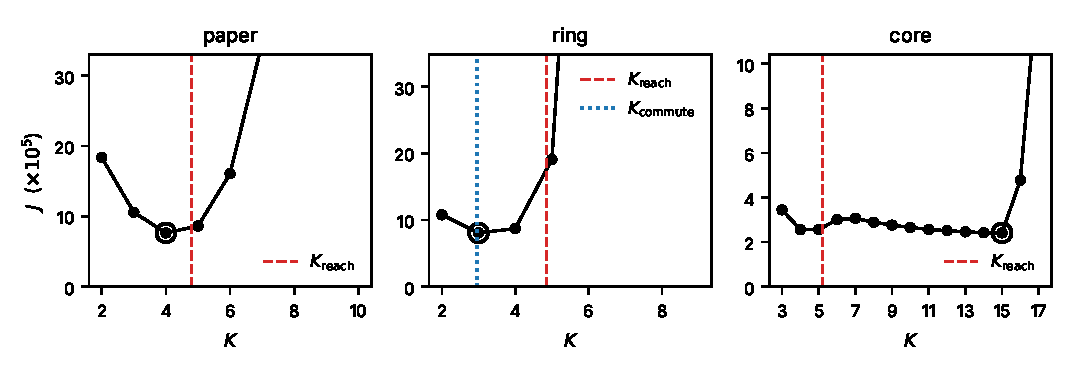
\includegraphics[width=.82\linewidth]{figs/fig_JvsK}
\caption{Mean $J(K)$ over the instances of a cell with the predicted caps (linear axes; the circled marker is the minimum of this cell-mean curve, not a per-instance optimum), $M=100$, $\Emax=1.5$~MJ. Paper: reach binds; $\lfloor\Kr\rfloor=4$ in 9 of the 12 instances. Ring: commute binds at $\Kc\approx3$, well below $\Kr=4.85$, with no abandonment at the optimum. Core: the reach cap is 5 ($\bar\ell=4.58$), but one abandoned sensor costs less than the served-set gain over the 12~h horizon, so the curve does not rise past it ($J=2.56$, $3.07$, $2.41$ and $4.77\times10^5$ at $K=4$, 7, 15 and 16); its minimum lies at $K=15$, against a mean per-instance optimum of $8.33$ (condition~\eqref{eq:window_apriori} and Proposition~\ref{prop:strand}).}
\label{fig:JvsK}
\end{figure*}

\begin{figure}[t]\centering
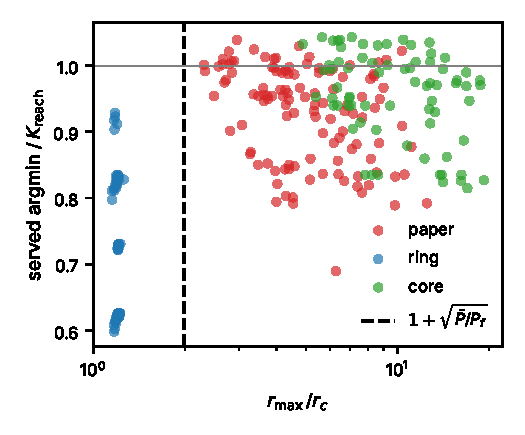
\includegraphics[width=\linewidth]{figs/fig_regime}
\caption{The fleet size minimising $J_{\mathrm{age}}$ among those at which every sensor is served, normalised by $\Kr$, against $\rmax/\rc$, with the boundary \eqref{eq:boundary}; 262 of the 272 instances (10 of the 12 clustered $M=400$ instances have no such fleet size). Instances left of the boundary optimise below $\Kr$ (commute-bound); right of it, 148 of 190 optimise at $\lfloor\Kr\rfloor$, 41 above it and 1 below.}
\label{fig:regime}
\end{figure}

\textit{Overall.} Across the 240 primary-grid instances (20 cells) the per-instance rule is exact in $55\%$ (95\% interval $[51,60]\%$) and within one UAV in $77\%$ ($[75,79]\%$); in 12 of 20 cells every instance is within one. The deviations are concentrated in two families and are not distributed noise: the 3~MJ \emph{ring} cells (the commute closed form under-predicts the annealer's optimum) and the \emph{core} family (criterion~\eqref{eq:window_apriori} flags), each analysed below. Excluding the seven cells with within-one agreement below $0.9$ --- ring at $M=50$ and $100$ (3~MJ), and core at $M=50$ (1.5~MJ), $M=100$ (both budgets) and $M=200$ (both budgets) --- the rule is exact in $73\%$ of instances ($[67,80]\%$) and within one in 155 of 156 ($[98,100]\%$). Replacing the full-buffer cap $\Kr$ by the flight-only cap $K_{\mathrm{flight}}$ of Section~\ref{sec:law:reach} raises exact agreement over the 240 instances from $0.55$ to $0.65$ and leaves within-one agreement at $0.77$; the paper-family bias (measured optimum minus rule, the sign used throughout) falls from $+0.23$ to $-0.04$. That gain assumes uninterrupted operation. To price it, we took six instances in which the choice matters and the flight-only cap wins, ran each at both fleet sizes over a 24~h horizon, and blocked every new launch for 3~h mid-run ($5$--$8$~h), as weather might; UAVs already airborne finish their sorties. Without the grounding the flight-only fleet size has $2$--$22\%$ lower AoI in all six. With it, the flight-only fleet size is $12$--$77\%$ worse in five of the six, and six of its seven gray-set sensors are never served again; at the robust cap the gray set is empty, so no sensor is at risk. The losses are the ones the survival threshold of Section~\ref{sec:law:reach} predicts: $b^{\star}_i(K)/B$ is $0.35$--$0.99$ for these seven sensors, the six with $b^{\star}_i(K)/\lambda_i$ shorter than the grounding ($0.9$--$2.6$~h) were lost, and the one with a longer margin ($4.1$~h) survived. We therefore keep the robust cap as the reach branch of the rule, and state the alternative as a condition an operator can check before deployment: the flight-only cap may be used when the longest service interruption the deployment must tolerate is shorter than $\min_{i\in\mathcal{G}}b^{\star}_i(K)/\lambda_i$ by at least a normal revisit interval.

\textit{Reach-bound, clustered fields.} In all eight paper cells the optimum lies within one UAV of the rule in every instance, with exact agreement 0.42--1.00 and the lower-side sign test significant in every cell. The 6~MJ cell, where revisits are frequent relative to event lifetimes, obeys the rule (mean optimum $19.25$ against $\bar\ell=18.67$; exact $0.42$, bias $+0.58$).

\textit{Commute-bound, spread fields.} In the three 1.5~MJ ring cells the served-set cost has an interior minimum at $K=3$ with zero abandonment while $\Kr\approx4.85$: the commute mechanism, not reach, sets the optimum, and the boundary \eqref{eq:boundary} classifies these cells correctly ($\rmax/\rc\approx1.2$ against $2.0$).

\textit{Two localised failure families.} The aggregate agreement figure is misleading, because the deviations are not scattered: the thirteen cells with within-one agreement of at least $0.9$ have mean bias $+0.38$ ($+5.3\%$ relative), exact agreement $0.73$ and within-one agreement $0.99$. The worst bias among them is $+2.08$, in core $M=50$, 3~MJ, which belongs to the core family but stays within one in 11 of 12 instances; among the other twelve it is $+0.67$ (ring $M=200$, 3~MJ). The remaining seven cells belong to the two families, with distinct mechanisms, analysed in Section~\ref{sec:eval:fail}.

\textit{A stated domain of validity.} Across the 14 reach-limited cells, relative bias correlates with $\rmax/\rc$ at $0.90$, and the cells fall into two groups: $-2\%$ to $+10\%$ for the eight clustered cells ($\rmax/\rc\le6.8$), with the core $M=50$, 3~MJ cell at $+21\%$ ($\rmax/\rc=6.0$), and $+42\%$ to $+178\%$ for the five core cells from $7.7$ upward ($+46\%$ and $+42\%$ at $7.7$, $+175\%$ at $12.6$, $+82\%$ at $13.6$, $+178\%$ at $16.2$). Since $\rmax/\rc$ is dimensionless, obtainable from a single pilot sortie, and already used to classify regime, it doubles as an empirical \emph{warning indicator}, calibrated on the measured commute radius (Section~\ref{sec:eval:exante} shows it does not transfer to an ex-ante estimate): beyond the level the rule degrades sharply, below it the rule is accurate to within $10\%$ on clustered fields, though not on every core cell. No cell lies between $6.8$ and $7.7$, so this grid places the warning level somewhere in that interval without fixing it. We deliberately avoid the word boundary, which this paper reserves for the analytical regime boundary \eqref{eq:boundary}; the level is an empirical observation of this study, not an analytical or fitted decision boundary. Five cells lie beyond it and all five degrade by a large margin. The level is the annealer's. C4, the cluster patrol and Liu et al.\ show the same jump at about $7.7$ (relative bias $+7\%$ to $+26\%$ there, $+52\%$ to $+122\%$ above $12$); Gao et al.'s bias stays within $+16\%$ up to $13.6$ and reaches $+76\%$ only at $16.2$; and Asghar et al.'s shows no jump at all, being high already below the level ($+22\%$ at $6.3$, $+44\%$ at $6.8$). As a warning against those planners' misses (optimum more than one UAV from $\ell$), the indicator and the design-time test \eqref{eq:window_apriori} perform alike (recall $0.49$ and $0.57$, precision $0.36$ and $0.33$, pooled over C4, the cluster patrol, Gao et al.\ and Asghar et al., with the level at $7.25$; across $(6.8,7.6)$ the indicator's recall is $0.48$--$0.51$); the misses neither catches are mostly the clustered- and ring-field deviations of planners whose optimum lies below $\ell$.

\subsection{The two failure families}\label{sec:eval:fail}
Both are now understood, and one of them yields a condition for when the coverage bound may be exceeded.

\textit{The reach cap bounds coverage, not optimality.} For $M=200$ in the core layout the rule gives $4.92$ while the measured optimum is $13.67$. Exactly one sensor of 200 is stranded from $K=5$--$7$ (depending on the instance) to $K=15$, and $J$ keeps falling well past that point ($6.64\times10^5$ at $K=4$ to $3.66\times10^5$ at $K=10$, with its minimum $3.27\times10^5$ at $K=14$). Stranding one sensor in 200 buys nearly three times the fleet. At 3~MJ the effect is larger still: the optimum is $28.42$ against a rule of $10.33$. This is a real trade-off, not a modelling error or an artefact of our planner --- the age-blind tour patrol also places the optimum far above the reach cap, at $11.00$ and $27.67$ for the two budgets (Sec.~\ref{sec:eval:baseline}) --- and Proposition~\ref{prop:strand} prices it. The precise location of the optimum once stranding pays is, however, planner-dependent: the annealer and the tour patrol agree to within one UAV at 3~MJ but differ by almost three at 1.5~MJ, and the cluster patrol, also age-blind, places the optima at $10.75$ and $15.58$.

\textit{Equal sharing is what makes this regime hard.} The core family is where a single long sortie matters most (Remark~\ref{rem:equal}), so we tested one departure from equal allocation. One UAV receives just enough energy to serve the peripheral sensor from any buffer state, $1.02\,(2\Pf\rmax/v+\Ph B/\Ru)$, and the other $K-1$ share the rest of $U$ equally; the inventory is unchanged, only its split. The funded UAV then plans freely like the others, so it serves the outlier on some sorties and core sensors on the rest. On core $M=100$ and $M=200$ at 1.5~MJ, 12 instances each, no sensor is stranded at the optimum in any of the 24 instances, and the AoI at the optimum falls by a median $53\%$ ($M=100$, lower in 12 of 12) and $20\%$ ($M=200$, 11 of 12) relative to equal shares. The optimum also becomes predictable again: it lies within one UAV of one plus the reach cap of the $K-1$ equally funded UAVs, which the second-farthest sensor sets, in 23 of the 24 instances and exactly in 14. The reach mechanism therefore appears to apply to whatever part of the fleet shares energy equally: the results suggest sizing one UAV's share for the outlier's full-buffer out-and-back and the remaining, equally funded fleet by the rule. We report this as an observation rather than a rule --- the split-fleet predictor was formed for this test and evaluated on two cells --- and general heterogeneous allocation remains open.

\begin{proposition}[Stranding condition]\label{prop:strand}
Let $\mathcal{S}(K)=\mathcal{S}_{\mathrm{guar}}(K)=\{i:r_i\le r_{\mathrm{reach}}(K)\}$ be the full-buffer surrogate served set and $Q_K=\sum_{i\in\mathcal{S}(K)}\sqrt{w_ic_i}$. Using Proposition~\ref{prop:sqrt} for the served set and charging each stranded sensor its age integral over the window, adding one UAV at fleet size $K$ lowers the \emph{surrogate} objective $J_{\mathrm{age}}^{\star}(C(K))+\sum_{i\notin\mathcal{S}(K)}w_i(T_b+T/2)$ if and only if
\begin{equation}\label{eq:strand}
\underbrace{\frac{Q_K^2}{2C(K)}-\frac{Q_{K+1}^2}{2C(K{+}1)}}_{\text{served-set freshness gained}}\;>\;\underbrace{\Big(T_b+\frac{T}{2}\Big)\!\!\sum_{i\in\mathcal{S}(K)\setminus\mathcal{S}(K+1)}\!\! w_i}_{\text{age cost of newly stranded sensors}},
\end{equation}
The sequential stopping point $\hat K$ is the smallest $K$ at which \eqref{eq:strand} first fails, capped at $\mathrm{round}\,\Kc$.
\end{proposition}
Three qualifications are deliberate. The condition inherits the full-buffer surrogate: sensors in the gray set $\mathcal{G}(K)$ are charged as stranded although a planner may keep them serviceable, so ``stranded'' here means ``without a full-buffer guarantee''. The condition governs the surrogate objective of Proposition~\ref{prop:sqrt}, not the planner's realised $J$. And $\hat K$ coincides with the global optimum only if the surrogate increments cross zero at most once in $K$. We have not proved that one-crossing property, so we report $\hat K$ as the sequential stopping point predicted by \eqref{eq:strand} rather than as $K^{\star}$ outright.
Equation~\eqref{eq:strand} is the one-step counterpart of the global surrogate test \eqref{eq:window_apriori}: $F(K)-F(K{+}1)$ is exactly the difference of its two sides, and the global test checks every larger fleet rather than stopping at the first failure. Every quantity in it is computable before deployment once $(\rc,\Pbar)$ are known (here they are measured): the sensor positions give $\mathcal{S}(K)$ and the radial surrogate $c_i^{\mathrm{rad}}=2\Pf r_i/v$ that we substitute for the true marginal cost, the weights are known, and $C(K)=\Pbar\,\Phi(K)$ is then closed-form. As elsewhere, using $c_i^{\mathrm{rad}}$ is an approximation: the ring analysis shows the true marginal cost moves with route composition, which sensor positions alone cannot capture.

Evaluated per instance on all 272 instances (24 cells), it does what it was derived to do and exposes its own limitation in the process (Table~\ref{tab:strand}). On the cell where the plain rule fails worst --- core, $M=200$, 1.5~MJ, where it predicts $4.92$ against a measured optimum of $13.67$ --- \eqref{eq:strand} predicts $14.00$, moving exact agreement from $0.00$ to $0.67$ and within-one agreement from $0.00$ to $1.00$; at 3~MJ it predicts $22.17$ against $28.42$ where the plain rule gives $10.33$. This supports the mechanism --- the optimum exceeds the coverage bound because one sensor's age integral is cheaper than the freshness bought for the other 199 --- but the size of the overshoot depends on the cost scale, as the next paragraph shows.

As a general-purpose point predictor, however, it is worse than the plain rule. Across all cells exact agreement falls from $0.56$ to $0.44$ and within-one agreement from $0.80$ to $0.77$: \eqref{eq:strand} removes the catastrophic tail in the core family but overshoots in the clustered family, increasingly with $M$ ($M=200$: $6.00$ against a measured $4.33$; $M=400$: $7.00$ against $4.42$, no instance within one). The reason is the cost scale. The gain term prices visits at $c_i^{\mathrm{rad}}$, about five times the measured energy per stop, so it over-states the freshness an extra UAV buys by the same factor, and since $Q_K^2$ grows as $M^2$ while the newly stranded weight does not, the over-statement grows with $M$. By Lemma~\ref{lem:scale}(ii), lowering the scale can only lower $\hat K$. At the measured scale the clustered overshoot disappears ($M=200$: $4.33$; $M=400$: $4.83$, every instance within one) and the agreement of \eqref{eq:strand} over all 272 instances rises to $0.58$ exact and $0.82$ within one, but the core cells are then under-predicted (core $M=200$, 1.5~MJ: $8.75$ against $13.67$, within one in 5 of 12), while both scales place the prediction above the coverage bound there. The surrogate therefore fixes the direction of the stranding trade-off but not its size; neither scale fits both families, and the planner's realised allocation, which Proposition~\ref{prop:sqrt} idealises, is a second source of error that we have not separated from the first. An earlier version of \eqref{eq:strand} held $Q$ fixed at $Q_K$ on both sides; that is not the surrogate difference, and it happened to offset part of this over-estimate (exact $0.52$, within-one $0.84$). We report the correct condition and its weaker numbers, and keep $\min(\lfloor\Kr\rfloor,\mathrm{round}\,\Kc)$ as the point predictor and \eqref{eq:strand} as the condition that says when the coverage bound may be exceeded. A gain term priced at the realised cost of a visit, which needs a pilot measurement, is the obvious next refinement. Its value as a predictor is also specific to the annealer. On the 82 held-out deployments the design-time test flags, the plain rule places the optimum of C4, the cluster patrol, Gao et al.\ and Liu et al.\ within one UAV in $79\%$, $76\%$, $80\%$ and $77\%$ of deployments, and \eqref{eq:strand} in only $54\%$, $45\%$, $35\%$ and $45\%$; only Asghar et al.'s class-based allocation agrees better with \eqref{eq:strand} ($44\%$ against $33\%$). Using \eqref{eq:strand} as the point predictor wherever the test flags therefore does not improve the rule, and we keep it as a condition rather than a predictor.

\begin{table}[t]\centering
\footnotesize\setlength{\tabcolsep}{3pt}
\caption{Coverage rule $\min(\lfloor\Kr\rfloor,\mathrm{round}\,\Kc)$ against the stranding condition \eqref{eq:strand}, selected cells and overall (272 instances, 24 cells).}
\label{tab:strand}
\begin{tabular}{lrrrrr}
\toprule
cell & measured & plain & \eqref{eq:strand} & plain $\pm1$ & \eqref{eq:strand} $\pm1$\\
\midrule
core $M{=}200$, 1.5~MJ & 13.67 & 4.92 & \textbf{14.00} & 0.00 & \textbf{1.00}\\
core $M{=}200$, 3~MJ & 28.42 & 10.33 & 22.17 & 0.08 & \textbf{0.17}\\
core $M{=}100$, 1.5~MJ & 8.33 & 4.58 & 8.75 & 0.67 & \textbf{0.92}\\
core $M{=}100$, 3~MJ & 14.00 & 9.83 & 11.42 & 0.83 & 0.83\\
paper $M{=}100$, 1.5~MJ & 4.25 & \textbf{4.25} & 5.00 & 1.00 & 0.92\\
paper $M{=}400$, 1.5~MJ & 4.42 & \textbf{4.00} & 7.00 & \textbf{1.00} & 0.00\\
ring $M{=}100$, 1.5~MJ & 3.00 & 3.00 & 3.00 & 1.00 & 1.00\\
\midrule
all cells: exact & & \textbf{0.56} & 0.44 & & \\
all cells: within one & & & & \textbf{0.80} & 0.77\\
\bottomrule
\end{tabular}
\end{table}


\textit{Ring at higher budget: the closed form, not the principle.} At 3~MJ the ring optimum lies at $6.7$--$8.5$ against $\Kc=6$, with no sensor stranded through $K=9$, so coverage plays no part. Measuring each factor separately localises the error precisely.

The \emph{principle} holds here. The measured fleet visit rate $1/T_{\mathrm{rev}}$ ($T_{\mathrm{rev}}$ the mean revisit interval), averaged over the cell, peaks at $K=8$ --- and so does the cell-mean $J$. Proposition~\ref{prop:sqrt}'s equivalence therefore holds for the cell-mean curves in the very cell where the closed form misses by two UAVs. What fails is $\Phi(K)$, the model of that rate, which peaks at $K=6$.

Three candidate causes are eliminated by measurement. The \emph{dwell} component of service time is ruled out by Proposition~\ref{prop:tau}, which shows it cancels identically; the hop component $\tau_{\mathrm{hop}}(K)$ is precisely what does not cancel and is treated below. The productive power $\Pbar$ is flat at $309$--$312$~W for $K\le9$, moving only once the fleet starts stranding sensors. And $\rc$ is flat within $4\%$ on the ring. What remains is the per-stop energy: the model's stop count $n=(\Eu-\Pf t_c)/(\Pbar\tau_s)$ under-predicts the realised count by a factor that \emph{grows} with $K$ (realised $26.9$ against $27.6$ at $K=4$, where the model is calibrated, and $10.5$ against $6.9$ at $K=8$: a ratio rising from $0.98$ to $1.53$, and to $1.63$ at $K=10$). Smaller budgets buy tighter clusters of stops whose intervening hops are shorter, so the marginal energy of a stop falls with $K$ while \eqref{eq:R} holds it fixed. This motivates a sublinear-yield diagnostic, but the per-sortie decomposition of Appendix~\ref{app:diag} shows the fitted exponent cannot be read as a hop-energy exponent; the operative correction is the $K$-dependent $\tau_{\mathrm{hop}}$ of Proposition~\ref{prop:tau}. A per-stop cost that decreases in $K$ shifts $\arg\max\Phi$ upward, in exactly the observed direction and of the observed size.

A fitted sublinear stop count $n=c(\Eu-\Pf t_c)^{\alpha}$ recovers part of the missing UAVs, but $\alpha$ is fitted, and Appendix~\ref{app:diag} shows it is an elasticity of the closed loop rather than a geometric constant, so we do not adopt it.



\textit{Horizon.} Table~\ref{tab:horizon} reports $J(24\,\mathrm{h})/J(12\,\mathrm{h})$. Below the reach cap the ratio is 0.98--1.02 (stationary); above it the ratio is 1.19--1.73 (the abandoned term grows with the window). This is the direct signature of the mechanism in Section~\ref{sec:law:reach}.

\begin{table}[t]\centering
\footnotesize\setlength{\tabcolsep}{3pt}
\caption{$J(24\,\mathrm{h})/J(12\,\mathrm{h})$, $M=100$, $\Emax=1.5$~MJ, six paired instances.}
\label{tab:horizon}
\resizebox{\columnwidth}{!}{%
\begin{tabular}{lccccccc}
\toprule
$K$ & 2 & 3 & 4 & 5 & 6 & 7 & 8\\
\midrule
paper ($\lfloor\Kr\rfloor=4$ in 9 of 12) & 0.98 & 0.99 & 1.00 & \textbf{1.19} & \textbf{1.46} & \textbf{1.56} & \textbf{1.58}\\
ring ($\Kc\approx3$, $\Kr=4.85$) & 1.02 & 1.00 & 0.99 & \textbf{1.19} & \textbf{1.73} & -- & --\\
\bottomrule
\end{tabular}%
}
\end{table}

\subsection{Fleet-sizing regret and the design-time criterion}\label{sec:eval:regret}
Agreement counts are a strict test of a discrete recommendation, but an operator cares how much freshness is lost by using the closed-form rule instead of sweeping $K$. Define the regret $\mathrm{Reg}=J(\ell)/J(K^{\star})-1$, with $\ell$ the rule's point prediction (also where the test flags). Two questions then matter: how large the regret is where the rule applies, and whether the operator can tell in advance where it does not. The design-time criterion \eqref{eq:window_apriori} is meant to answer the second, so we apply it to every instance and report regret conditional on its verdict (Table~\ref{tab:regret}).

\begin{table}[t]\centering
\footnotesize\setlength{\tabcolsep}{3pt}
\caption{Fleet-sizing regret $J(\ell)/J(K^{\star})-1$, conditional on the design-time criterion \eqref{eq:window_apriori}. Commute-bound instances (ring) are classified by the boundary \eqref{eq:boundary}, to which the window test does not apply.}
\label{tab:regret}
\resizebox{\columnwidth}{!}{%
\begin{tabular}{llrrrrr}
\toprule
family & test & $n$ & median & 90th pct & max & $<5\%$\\
\midrule
paper & pass & 49 & 0.0\% & 5.0\% & 14.8\% & 90\%\\
paper & flagged & 47 & 0.0\% & 5.4\% & 11.1\% & 89\%\\
core & pass & 24 & 0.0\% & 21.6\% & 26.4\% & 58\%\\
core & flagged & 48 & 24.1\% & 118.9\% & 167.8\% & 25\%\\
ring & (commute-bound) & 72 & 0.4\% & 21.8\% & 27.4\% & 62\%\\
\midrule
all reach-bound, test passes &  & 73 & 0.0\% & 11.4\% & 26.4\% & 79\%\\
all reach-bound, flagged &  & 95 & 0.8\% & 80.2\% & 167.8\% & 57\%\\
\bottomrule
\end{tabular}%
}
\end{table}

Three things follow. First, in the clustered family the rule is an essentially free substitute for an exhaustive sweep: half the instances lose nothing and nine in ten lose under $5\%$. Second, empirically the test behaves as intended: no reach-bound instance whose regret exceeds $27\%$ passes, and every instance above $30\%$ is flagged (all 23 of them are reach-bound)---the 48 core instances it flags have median regret $24\%$, the 24 it passes have median $0\%$---while its false alarms are cheap: the 47 paper instances it flags have $90$th-percentile regret of $5\%$ (at most $11\%$). An operator who runs the test and, when it flags, sweeps $K$ instead of trusting the rule loses little in the reach-bound families: where the test passes the regret is a median $0\%$, $11\%$ at the 90th percentile and at most $26\%$. Third, the commute-bound family's regret is a different quantity: the boundary \eqref{eq:boundary} classifies these instances correctly, and their median $0.4\%$ and maximum $27\%$ are the price of the constant-cost closed form \eqref{eq:Kcommute}, recoverable by maximising the measured visit rate (Sec.~\ref{sec:eval:fail}) and not by a better commute radius: the ex-ante inputs of Sec.~\ref{sec:eval:exante} leave these instances' predictions, and therefore their regret, unchanged. We report these separately: a pooled figure would flatter the rule where it works and hide where it does not. The flatness that makes the commute optimum hard to pin down is also what makes missing it cheap: at $M=40$ the cheaper of the two neighbouring fleet sizes costs a median $3.2\%$ in $J$ on the ring, against $22\%$ in the clustered family, and the same holds under the tour patrol ($3.1\%$ against $18\%$) and CP-SAT ($3.7\%$ against $19\%$) (Sec.~\ref{sec:eval:baseline}), though not under the cluster patrol ($19.6\%$ on the ring against $14.2\%$ clustered).

\subsection{Scaling in field size}\label{sec:eval:L}
Both caps scale nearly as $vU/(\Pf\cdot\text{length})$, so $K^{\star}\approx\propto1/L$ at fixed $\Emax$. Table~\ref{tab:L} tests this axis directly, which the $\Emax$ sweep cannot: $\Emax$ and $L$ enter the rule essentially only through the ratio $U/L$, so varying $\Emax$ alone cannot distinguish the rule from any other quantity proportional to $U$. Table~\ref{tab:L} gives the result. The optimum falls monotonically from $7.25$ to $3.00$ as $L$ goes from 8 to 20~km and the rule tracks it from $7.00$ to $2.88$, with mean bias $+0.41$ over the 32 field-size instances and \emph{every} instance within one UAV at every field size. The exact-agreement dips at 10 and 16~km have different causes. At 8 and 10~km every miss sits at $\lfloor K_{\mathrm{flight}}\rfloor$, inside the reach bracket (regret $1$--$18\%$); at 16 and 20~km the optimum lies above $K_{\mathrm{flight}}$ with 1--3 sensors never served, the finite-window trade-off (regret $3$--$17\%$, and $39\%$ for the one miss at 20~km). Scaling the field scales $\rmax$ and $\rc$ together, so $\rmax/\rc$ stays in $5.5$--$6.8$ and every cell remains reach-limited; this sweep therefore varies the magnitude of the optimum over a $2.4\times$ range without changing regime, which is what makes it a clean test of scaling.

\begin{table}[t]\centering
\caption{Field-size sweep, paper layout, $M=100$, $\Emax=1.5$~MJ, 8 instances per $L$ (12 at 12.6~km).}
\label{tab:L}
\small
\begin{tabular}{lccccc}
\toprule
$L$ (km) & 8 & 10 & 12.6 & 16 & 20\\
\midrule
measured $\arg\min_K J$ & 7.25 & 5.88 & 4.25 & 3.88 & 3.00\\
rule & 7.00 & 5.25 & 4.25 & 3.25 & 2.88\\
exact agreement & 0.75 & 0.38 & 1.00 & 0.38 & 0.88\\
within $\pm1$ & 1.00 & 1.00 & 1.00 & 1.00 & 1.00\\
$\rmax/\rc$ & 5.5 & 6.1 & 6.3 & 6.8 & 6.3\\
\bottomrule
\end{tabular}
\end{table}

\subsection{Depot position}\label{sec:eval:depot}
Every result so far places the depot at the centre of the field. Moving it changes nothing in the rule's form --- $\rmax$ and $\rc$ are measured from the depot --- but it changes the geometry the rule has to summarise. We repeated the grid for all three families with the depot at $(0.25L,0.25L)$ (216 instances) and for the paper and ring families with it near an edge midpoint, $(0.10L,0.50L)$ (48 instances), with the same protocol and the same anti-censoring extension, on the union $K$ grid of the three depot planners, which lengthened 122 of the 264 annealer sweeps (Table~\ref{tab:depot}). The layouts stay centred on the field and only the depot moves, so at the quarter-point depot the outlier is not the farthest sensor in 9 of the 36 core fields (18 of 72 instances).

\begin{table}[t]\centering
\footnotesize\setlength{\tabcolsep}{3pt}
\caption{The rule with an off-centre depot. Bias is measured optimum minus rule; regret is $J(\ell)/J(K^\star)-1$.}
\label{tab:depot}
\begin{tabular}{llrrrrr}
\toprule
depot & family & $n$ & exact & $\pm1$ & bias & regret med / p90\\
\midrule
$(0.25L,0.25L)$ & paper & 72 & 0.85 & 1.00 & $+0.07$ & 0.0 / 5.6\%\\
 & core & 72 & 0.61 & 0.89 & $+0.29$ & 0.0 / 16.8\%\\
 & ring & 72 & 0.25 & 0.96 & $-0.79$ & 9.2 / 21.7\%\\
\midrule
$(0.10L,0.50L)$ & paper & 24 & 0.88 & 1.00 & $-0.12$ & 0.0 / 0.8\%\\
 & ring & 24 & 0.00 & 1.00 & $-1.00$ & 22.3 / 40.7\%\\
\bottomrule
\end{tabular}
\end{table}

The reach mechanism carries over: on the clustered and core layouts the rule is as accurate as with a central depot or more so, although on the core layout the outlier no longer always sets $\rmax$; ex-ante commute inputs change the rule in 3 of the 72 core instances, all toward the optimum. The ring does not carry over. There the rule is one UAV too high in 51 of 72 instances at the quarter point and in all 24 near the edge, and the error grows with the offset, from a median regret of $9\%$ at the quarter point to $22\%$ near the edge. The ring is centred on the field, so an off-centre depot sees its near side at a few kilometres and its far side five to nine times farther ($2.3$ against $12.2$~km at the quarter point). The far side binds through commute cost --- a sortie there spends most of its energy getting there and back --- but the rule's commute radius is a fleet average dominated by cheap near-side sorties, so $\Kc$ is overestimated, never binds, and the rule falls back on $\lfloor\Kr\rfloor$, one UAV too many. The rule has no notion of a commute radius that varies across the field, and a central depot never exposed that. The planner comparison transfers: under the same measurement rule the territorial scheduler of Section~\ref{sec:eval:baseline} lowers the published method's own-optimum $J$ at the quarter-point depot by a median $13.9\%$ (core, 72 of 72), $22.6\%$ (paper, 72 of 72) and $7.6\%$ (ring, 65 of 72), and near the edge by $23.4\%$ (paper, 24 of 24) and $2.4\%$ (ring, 20 of 24), the last a small margin. The rule still lies within one UAV of the annealer's optimum in $89$--$100\%$ of these instances per family, but in the tested off-centre ring deployments the point prediction is consistently biased upward, by about one UAV.

\subsection{Coordination}\label{sec:eval:coord}
Table~\ref{tab:coord} compares the coordinated fleet with the same planner given only the age vector (no commitments). Without coordination, 35--71\% of visits arrive at a sensor another UAV reset after the visiting UAV planned it (rising with $K$). The objective is $2.9\times$ worse at $K=4$ and $2.7\times$ worse comparing each variant at its own optimum, and, because the waste grows with $K$, the measured optimum shifts from a mean of $4.25$ to $3.58$. Coordination is therefore not a refinement but a prerequisite for measuring $K^{\star}$ at all. The mechanism requires only that each UAV report its route to the depot at launch.

\begin{table}[t]\centering
\footnotesize\setlength{\tabcolsep}{3pt}
\caption{Mean $J$ ($\times10^{5}$), paper, $M=100$, $\Emax=1.5$~MJ, 12 instances.}
\label{tab:coord}
\begin{tabular}{lccccccc}
\toprule
$K$ & 2 & 3 & 4 & 5 & 6 & 7 & 8\\
\midrule
coordinated, launch-time SA & 18.4 & 10.6 & \textbf{7.6} & 8.6 & 16.1 & 34.6 & 62.5\\
uncoordinated & 25.8 & \textbf{20.5} & 22.3 & 25.0 & 39.7 & 57.3 & 78.3\\
duplicate-visit fraction & .35 & .46 & .56 & .58 & .64 & .68 & .71\\
coordinated, per-leg SA & 18.6 & 11.2 & \textbf{8.3} & 9.5 & 16.6 & 35.0 & 62.8\\
\bottomrule
\end{tabular}
\end{table}

\subsection{Per-leg replanning and mid-leg diversion}\label{sec:eval:replan}
Re-optimising the remaining route after every stop nearly eliminates sortie truncation (from up to $5.8\%$ of sorties, at $K=2$, to at most $0.1\%$) but raises $J$ by $0.5$--$9.9\%$ over $K=2$--$8$ ($8$--$10\%$ at $K=4$--$5$) when the per-leg re-optimisation is given one twentieth of the launch-time budget (60 versus 1200 iterations). The optimum is unchanged in 11 of the 12 instances. The comparison is computationally confounded --- per-leg decisions get 60 annealing iterations against 1200 at launch --- so the finding is that \emph{under this computational allocation} frequent replanning does not pay, not that replanning is intrinsically valueless. What is robust is that the measured $K^{\star}$ is essentially unchanged.

\textit{Mid-leg diversion.} Per-leg replanning still commits a UAV to the leg it is currently flying. A natural question is whether a UAV should abandon that leg when the fleet state changes in transit. Note first that the coordination rule already removes the adversarial case: because a committed sensor is withdrawn from every other planner's candidate set, the first UAV to commit keeps its target and cannot be pre-empted en route. What remains is opportunity cost---another sensor's age grows, or an event fires there, while the UAV is between stops. We implemented diversion to test it: whenever a UAV replans after a stop, every other UAV in flight re-evaluates from its current position and abandons the current leg if an alternative target exceeds the committed one by a factor $\mu$ (a margin that prevents oscillation between two targets); the energy already spent on the abandoned leg is charged, the pending arrival is cancelled and a new one scheduled from the current position. With $\mu=1.25$ it changes the objective by $+0.7\%$ relative to per-leg replanning alone, worse in 8 of 12 paired instances ($p=.39$; Table~\ref{tab:ablation}): we detect no value in abandoning a leg.

\subsection{How $\rc$ varies with fleet size}\label{sec:eval:rc}
Measuring $\rc$ against $K$ across all 20 primary cells confirms the order-statistic prediction of Section~\ref{sec:law:commute}: $\rc$ \emph{rises} with $K$ by more than $5\%$ over the swept range in 14 of the 20 cells and is flat (within $4\%$) in the six ring cells. The rise is $22$--$72\%$ in the clustered family and $11$--$88\%$ in the core family; on the ring $\rc$ falls slightly, by $3$--$4\%$, where the i.i.d.\ order-statistic model predicts it flat or rising, so this small fall is the planner's.

This has a consequence for what a corrected $\rc(K)$ could buy, and it is not what one would expect. The two families in which the rule misses (Section~\ref{sec:eval:fail}), the 3~MJ ring and the core layout, are exactly those in which such a correction cannot act: on the ring, where $\Kc$ binds, $\rc$ is flat, so the correction is near zero; in the core family, as in the clustered one, $\rc$ varies most but $\Kc$ is far from binding ($36.3$, and $15.5$ for clustered, against $\Kr\approx5$ at $M=100$, 1.5~MJ), so the correction changes an inactive term. We therefore state the $\rc(K)$ dependence as a bound on the closed form's accuracy rather than presenting a corrected form, and locate the two failures in their own mechanisms instead.

\subsection{Predicting $\rc$ before deployment}\label{sec:eval:exante}
$\Kc$ uses the realised commute radius, which we measure from the runs. That is legitimate for validating the mechanism but circular as a design rule. Two routes make it non-circular, and neither needs a fleet sweep. The order-statistic form $\mathbb{E}[\rc\,|\,n]\approx\tfrac12(\mathbb{E}r_{(1)}+\mathbb{E}r_{(2)})$ of Section~\ref{sec:law:commute} requires only the radial distribution $F_r$ of the deployment, known from the site survey that fixes where sensors go, together with $n$ from the energy budget, and so gives $\hat\rc$ from geometry. It is exact for the nearest two of $n$ i.i.d.\ radial draws, which the planner's stops are not --- they are selected on age, priority, route cost and commitments --- so it is an i.i.d.\ order-statistic \emph{approximation} whose accuracy is itself to be tested, not a planner-independent property of the route. Alternatively a single pilot sortie at the largest candidate $\Eu$ returns $\rc$ directly, at the cost of one flight rather than a fleet sweep; we evaluate the first route, which needs no flight at all.

We compute every commute input from the site survey, the airframe, the sensors' nominal rates and the inventory, with no flight and no fleet sweep. $\hat\rc$ is the order statistic above with $F_r$ the empirical radial distribution of the sensors. $\hat n$ comes from the energy budget, $n=(\Eu-\Pf t_c)/(\Pbar\tau_s)$, with the inter-stop time taken from the mean nearest-neighbour spacing of the sensors. $\hat{\Pbar}$ comes from the conservation law of Proposition~\ref{prop:tau}: the fleet hovers $H=\sum_i\lambda_i/\Ru$ UAV-equivalents, so the hover share of productive time is $h=H/(K(1-t_c/T_s))$ and $\Pbar=\Pf+(\Ph-\Pf)h$. We evaluate them at the smallest candidate fleet size $\lfloor0.5\Kr\rfloor$, where the measured values used elsewhere in the paper are taken; this is the pre-deployment estimator. A self-consistent alternative, the commute fixed point $K=\Kc(\hat\rc(K))$, does not exist in most instances: the map jumps across the diagonal where $\hat n$ reaches its floor of one stop, in 151 of the 272 instances, so we do not use it. Over all 272 instances:
\begin{itemize}
\item \emph{The point predictor is unchanged.} Ex-ante inputs change it in none of the 272 instances, so its agreement ($0.56$ exact, $0.80$ within one) and regret are exactly those reported with measured inputs, and the regime classification by \eqref{eq:boundary} agrees in every instance.
\item \emph{The design-time criterion keeps its properties.} With ex-ante inputs \eqref{eq:window_apriori} changes its verdict on 3 of the 168 reach-bound instances, all toward flagging. No passing reach-bound instance loses more than $27\%$, every instance above $30\%$ is still flagged, and the paper-family pass rows keep a 90th-percentile regret of $5\%$. The interval $[K_0,K_R]$ that Result~1 returns when the test flags a field, computed from ex-ante inputs, contains the measured optimum in 167 of 168 reach-bound instances, as with measured inputs.
\item \emph{$\hat{\Pbar}$ is accurate.} It tracks the measured value with correlation $0.976$ and mean error $1.4$~W over a measured range of $303$--$339$~W, against $7.4$~W for the best constant.
\item \emph{$\hat\rc$ is accurate only where it matters.} Compared at the smallest candidate fleet size, where the measured value is taken: on the ring it is $0.94$--$0.96$ of the measured value (10th--90th percentile). In clustered and core fields it is well below it, a median $0.61$ and $0.44$ of the measured value, and still $0.79$ and $0.49$ with the measured $n$: the planner's first and last stops are not the nearest two of $n$ random draws. On clustered fields $\hat n$ adds to the error: it is about twice the measured value, the nearest-neighbour spacing understating real hops, which lowers $\hat\rc$ further and feeds $\hat{\Pbar}$.
\end{itemize}
The estimator needs to be accurate only where its input controls the decision, and the reason is structural. There the reach cap binds and $\Kc$ is far above it; an under-estimated $\hat\rc$ only raises $\hat\Kc$ further, and it only moves $\rmax/\rc$ further from the boundary \eqref{eq:boundary}. The commute cap binds only where sensors avoid the neighbourhood of the depot, which is also where the nearest of $n$ radii is a good estimate of the commute radius. We have tested this on one commute-bound family, and do not claim it for commute-bound fields in general. The one quantity that does not survive is the warning indicator of Section~\ref{sec:eval:law}: with $\hat\rc$ every reach-limited cell exceeds the warning level (the smallest ex-ante cell-mean ratio is $8.1$), and the six core cells read $22$--$25$ whatever their bias, so that indicator requires a measured commute radius, from a pilot sortie, and is not a pre-deployment test.

\textit{Sensitivity to the known inputs.} Estimating the commute inputs is one source of error; the physical inputs the rule takes as known are another. Misstating one of them changes only the prediction, not the system, so we score the rule computed from a perturbed input against the recorded $J(K)$ of every deployment. The rule is insensitive to $\Ph$ and $\Ru$, which enter only through the small hover term: a $\pm20\%$ error leaves within-one agreement at $0.77$. It is sensitive to $U$, $\Pf$ and $\rmax$, because $\Kr$ scales exactly with $U$ and nearly with $1/(\Pf\rmax)$: a $10\%$ error in $U$ moves it by $10\%$ and one in $\Pf$ or $\rmax$ by $9.3$--$9.8\%$, one or two UAVs in this grid; exact agreement falls to $0.26$--$0.37$ and median regret rises to $7$--$13\%$. The cost is asymmetric. Errors that overstate the fleet push it past the reach cap, where sensors are stranded, and have a 90th-percentile regret of $137$--$148\%$; errors in the conservative direction cost $37$--$46\%$. This sensitivity belongs to energy-limited fleet sizing rather than to the rule: a fleet sweep in a simulator given the same energy parameters would err similarly. The practical consequence is that the energy per sortie and the farthest sensor distance must be known to within a few percent, and that an operator unsure of them should err toward less energy and longer distance.

\subsection{Robustness of the optimum to the planner}\label{sec:eval:baseline}
Every comparison so far varies our own planner, which cannot establish that the measured optimum is a property of the problem rather than of that planner. We therefore measure it under four other planners: three that share nothing with the annealer except the simulator, the energy accounting and the coordination protocol, and CP-SAT, which solves the annealer's own per-decision problem \eqref{eq:sortie} with the same hover estimate. Each honours the commitment set of Section~\ref{sec:model:coord}, so none gains or loses from duplicate visits.
\begin{itemize}
\item \emph{Tour patrol.} One closed tour through the depot and every sensor (nearest-neighbour construction, then 2-opt) is cut into consecutive sorties by the energy budget: a shared pointer advances around the tour and each launching UAV takes the next run of sensors that fits, skipping sensors committed elsewhere or unreachable on their own. Ages and priorities play no part in selection; they enter only through hover budgeting. This is route-first, cluster-second routing, and what an operator would deploy without this work. It is also the energy-constrained form of the shared-tour policy of \cite{rahimi2024graph}, in which UAVs are spread along one tour through every sensor and circulate on it; their model has no depot or energy budget, so here the tour is cut into sorties that fit it.
\item \emph{Sweep patrol.} The same, with the tour replaced by polar angle about the depot.
\item \emph{Cluster patrol.} The clustering stage of the method of \cite{rahimi2024graph} (its tour merging and path post-optimisation are omitted): the sensors are partitioned by $k$-means into one cluster per UAV, and each UAV patrols a closed tour of its own cluster, cut into energy-feasible sorties as above. As in the original, ages and priorities play no part in selection; unlike the shared-tour patrols it gives every UAV a fixed territory.
\item \emph{CP-SAT.} The per-decision problem \eqref{eq:sortie} solved by constraint programming, as in Section~\ref{sec:planner:cert}, cold-started and with a deterministic search budget, so that results do not depend on machine load. It proves $96.6\%$ of $43{,}426$ decisions optimal at its default budget.
\end{itemize}

\begin{table}[t]\centering
\footnotesize\setlength{\tabcolsep}{3pt}
\caption{Fleet-size optimum under independent planners. Top: primary grid, 216 paired instances ($M\le200$, $\Emax\le3$~MJ: 18 cells), per-instance argmin on the common $K$ range. In every row the rule's $\ell$ is the planner-independent one, computed from the annealer's smallest-$K$ commute inputs. Bottom: controlled comparison at $M=40$, $\Emax=1.5$~MJ, paper and ring layouts, 12 instances each. ``$=$'' exact agreement, ``$\pm1$'' within one UAV. Agreement with the rule is computed directly, not by transitivity.}
\label{tab:baseline}
\begin{tabular}{lrrrr}
\toprule
planner & $=$SA & $\pm1$ SA & $=$rule & $\pm1$ rule\\
\midrule
annealer (SA, ours) & -- & -- & 0.56 & 0.75\\
tour patrol & 0.61 & 0.92 & 0.53 & 0.79\\
sweep patrol$^{\ast}$ & 0.56 & 0.92 & 0.56 & 0.85\\
cluster patrol \cite{rahimi2024graph}$^{\dagger}$ & 0.47 & 0.71 & 0.50 & 0.84\\
territorial scheduler (C4, ours)$^{\dagger}$ & 0.55 & 0.83 & 0.52 & 0.88\\
Gao et al.\ \cite{gao2023aoi}$^{\dagger}$ & 0.31 & 0.61 & 0.38 & 0.76\\
Asghar et al.\ \cite{asghar2025persistent}$^{\dagger}$ & 0.21 & 0.62 & 0.26 & 0.64\\
Liu et al.\ \cite{liu2022aoi}$^{\dagger}$ & 0.54 & 0.77 & 0.55 & 0.86\\
\midrule
\multicolumn{5}{l}{$M=40$, 24 instances}\\
annealer (SA, ours) & -- & -- & 0.67 & 1.00\\
tour patrol & 0.75 & 1.00 & 0.75 & 1.00\\
CP-SAT & 0.75 & 1.00 & 0.67 & 1.00\\
cluster patrol & 0.50 & 0.88 & 0.42 & 0.96\\
\bottomrule
\end{tabular}
\par\smallskip{\footnotesize $^{\ast}$paper and ring only; SA on the same 144 instances: 0.67 / 0.84 against the rule. CP-SAT: default search budget on paper; threefold budget on ring, where it is converged (see text). $^{\dagger}$own optima on the union $K$ grid of all compared planners, uncensored.\par}
\end{table}

\textit{The optimum moves less than the objective.} Table~\ref{tab:baseline} gives the result. The tour patrol's optimum lies within one UAV of the annealer's in $92\%$ of instances ($[89,94]\%$), and the sweep patrol's in $92\%$ of those it covers ($[88,96]\%$); at $M=40$ all three planners lie within one UAV of each other and of the point predictor in all 24 instances, which bounds the rate below by $86\%$ at 95\% confidence. Figure~\ref{fig:planners} shows the $M=40$ curves. The rule predicts the tour patrol's optimum about as well as it predicts ours ($0.53$ / $0.79$ against $0.56$ / $0.75$). This is not because the planners perform alike. The tour patrol is $25\%$ worse than the annealer on clustered fields and $11\%$ \emph{better} on the ring, and the sweep patrol is more than twice as costly on clustered fields; CP-SAT improves on the annealer by $5.9\%$ at $M=40$. Which planner achieves the lower AoI depends on the geometry, yet the fleet size each would recommend is, in most regimes, the same.

\textit{A published competitor.} The cluster patrol is the most different of these planners, and the only one with fixed territories. On AoI neither it nor the annealer dominates. At each planner's own optimum the cluster patrol's median $J$ is $36\%$ higher on clustered fields (the annealer's is lower in 61 of 72 deployments), while the cluster patrol's is $4\%$ lower on the ring (51 of 72) and $29\%$ lower on the core layout (55 of 72); at matched fleet sizes the two differ by $0.1\%$ in median over all 3{,}162 runs. On the representative cell (paper, $M=100$, 1.5~MJ) the annealer's mean $J$ is lower at every fleet size swept, by $36\%$ at $K=4$. The two win through different mechanisms, which the rate--allocation--regularity decomposition described at the end of this section separates (two instances per layout, $M=100$, outside the evaluation seeds). On the core layout the cluster patrol's fixed loops revisit every sensor at an exactly constant interval, losing nothing to irregular revisits, and its hops are shorter ($17$ against $25$~s); irregular revisits inflate the annealer's objective by $19$--$20\%$ ($E_{\mathrm{reg}}$). On the clustered layout the annealer wins through commute efficiency: sharing the whole field, most of its sorties stay near the depot's dense area (commute radius $0.8$--$1.9$~km against $4.0$--$4.7$~km for fixed territories), which gives it $47\%$ more visits per hour. Allocation by priority is not the lever in either case: with priorities spread over $[1,10]$, even the ideal square-root allocation is worth at most $7\%$ over visiting every sensor equally often. Fixed territories buy regularity at the price of commute; field-wide scheduling buys commute efficiency at the price of regularity. Its fleet-size optimum is less close to the annealer's --- within one UAV in $71\%$ of deployments ($[66,76]\%$), on average $1.9$ UAVs smaller and $4.0$ smaller on the core family, where the finite-window optimum is already known to depend on the planner (Section~\ref{sec:eval:fail}) --- but closer to the rule: within one UAV of the point predictor in $84\%$ ($[80,88]\%$), more often than the annealer's by $9.7$ points (paired, $[5.6,13.9]$). At $M=40$ it is within one UAV of the rule in 23 of 24 instances. A published policy with a different structure, fixed territories instead of shared age-aware scheduling, therefore reaches an optimum the rule predicts at least as well as ours. The cluster patrol is the exception to a pattern the tour patrol shows clearly: the tour patrol and the annealer, whose $J$ differs by up to $25\%$, agree more closely with each other about $K^{\star}$ than either does with the closed form, and the difference is significant as a paired comparison on the same deployments --- the rate at which they lie within one UAV of each other exceeds the rate at which the annealer lies within one of the rule by $17.1$ points (95\% interval $[14.3,20.4]$), and the tour patrol's by $12.5$ points ($[9.3,15.7]$). The cluster patrol instead agrees more often with the rule than with the annealer.

\textit{A planner built from the comparison.} The diagnosis above suggests keeping fixed territories, which buy regularity, while choosing them to cut commute. We built such a planner, a depot-aware territorial scheduler (C4). Each UAV owns a disjoint sensor set and flies a fixed cyclic visit sequence, cut into energy-feasible sorties at launch by the same rule as the cluster patrol. The sets and tours are chosen before deployment by local search --- relocating sensors between UAVs, re-optimising tours, assigning frequency classes --- on a per-UAV simulation surrogate that uses only planner-side information: positions, priorities, system parameters and nominal generation rates. The surrogate scores a design over the same burn-in and horizon as the evaluation ($3$ and $12$~h), without events and with nominal rather than realised rates, so a design is tuned to the operating window it will be judged on, as an operator would tune it to a planned deployment; a different window needs a new search. The search starts from the published $k$-means partition and from equal angular sectors and deploys whichever the surrogate prefers; without search, the first start reproduces our adaptation of the published method exactly. Unlike the published method, and like the annealer, it uses priorities. It was designed on separate pilot seeds with every setting fixed in advance, and evaluated once on the 216 held-out deployments against a criterion registered beforehand: a median own-optimum $J$ below the cluster patrol's in \emph{each} family, with own optima taken on the union of both planners' $K$ values and extended until each planner's three largest $K$ values exceed $1.5$ times its minimum, so that no optimum is censored. A defect in the surrogate's clock surfaced during the first evaluation attempt; it was reproduced and fixed on pilot data, and the evaluation was rerun from scratch with no comparative statistic computed in between. The criterion holds in every family. Median own-optimum $J$ is $24.7\%$ lower on clustered fields ($[19.0,26.7]\%$, all 72 deployments), $10.3\%$ lower on the core layout ($[9.3,12.0]\%$, all 72) and $5.9\%$ lower on the ring ($[3.3,7.3]\%$, 61 of 72), 205 of 216 overall. The ring is the thin case: one ring cell ($M=100$, 1.5~MJ) is a tie ($-0.8\%$, 6 of 12), and the largest single loss is $8.4\%$. At the rule's fleet size $\ell$ instead of each planner's own optimum the margins are $26.6$, $10.4$ and $3.1\%$, so the gain is not a by-product of choosing a different $K$. The partition carries part of it on clustered fields, where equal sectors without search already beat the published method by $7.9\%$ (53 of 72 deployments), about a third of C4's margin there; on the core ($+10.8\%$) and ring ($+2.8\%$) layouts they lose to it, so the gain there comes from the surrogate-guided search, and frequency classes are nearly inert (a median $2\%$ of sensors leave the base class). Two other designs failed: a selector choosing between planners by regime separated the synthetic families rather than the regimes and broke with an off-centre depot, and three hybrids (the annealer within territories, a square-root-due patrol, balanced territories) were each worse than one of their parents, and a quadratic age index in the annealer is $7.2\%$ worse than the linear one (Table~\ref{tab:ablation}). For fleet sizing, the stronger planner's optimum is predicted at least as well as the published one's: within one UAV of the point predictor in $88\%$ of deployments (exactly in $52\%$), against $84\%$ ($50\%$) for the cluster patrol, and in $96\%$ on clustered fields, $11.1$ points above the cluster patrol there ($[2.8,19.4]$). Against the annealer, in a secondary comparison registered with the criterion but not part of it, the result is mixed. The median of $J^{\star}_{\mathrm{C4}}/J^{\star}_{\mathrm{SA}}-1$ is $-40.4\%$ on the core layout ($[-45.9,-31.4]\%$, C4 lower in 72 of 72 deployments) and $-9.9\%$ on the ring ($[-13.0,-7.3]\%$, 64 of 72), but on clustered fields it is $-1.8\%$ with an interval that includes zero ($[-11.0,+3.6]\%$, 42 of 72), and the annealer wins two of the three clustered cells at 1.5~MJ outright, by $17.0\%$ at $M=100$ (11 of 12 deployments) and $30.3\%$ at $M=200$ (12 of 12); at $M=50$ C4 is $7.3\%$ lower (12 of 12). C4 therefore does not supersede the annealer: field-wide, age-driven scheduling remains preferable on clustered fields with $M\ge100$ under tight energy, the same split by mechanism as between the annealer and the published method. The two planners' optima lie within one UAV of each other in $83\%$ of deployments. Both were measured under the same rule, and C4 is deterministic across machines (to one unit in the last place), so its runs are comparable with the annealer's, which all come from one machine.

\textit{Two recent methods from IEEE journals.} We also adapted two recent published methods: Gao et al.\ \cite{gao2023aoi}, which partitions sensors into territories by kernel $k$-means with the depot in every centroid and routes each UAV by ant-colony optimisation to minimise sink-side average and peak AoI, and Asghar et al.\ \cite{asghar2025persistent}, which plans persistent cyclic coverage to minimise the maximum weighted revisit time, the peak form of our objective; we implement its fixed-fleet, recharge-constrained variant. Both were implemented from the published versions and adapted to continuous operation from one depot with the energy inventory divided among $K$ airborne UAVs, $K$ an input and swept. Every unspecified detail was fixed before the held-out evaluation and is listed in the code. Gao et al.\ first group sensors into collection points; because our UAVs collect by hovering over each sensor, every sensor is its own collection point, the one-to-one configuration that paper also evaluates. Its kernel is not given (we use a linear one) and its ant-colony settings are the published ones; Asghar et al.'s rooted cycle covers are solved by CP-SAT where the paper uses an integer program. Both plan offline from planner-side information and fly the plan cyclically, one planned trip per sortie, with a launch-time feasibility check against the live dwell estimate; the planned dwell (at the planned revisit interval rather than a full buffer) was chosen on pilot seeds by a rule registered in advance and in each method's favour ($19.8\%$ and $9.6\%$ lower $J$ than the alternative). Both methods therefore optimise a different objective than ours and plan with a fixed dwell estimate, which costs them against the live-dwell planners; Asghar et al.'s class-based allocation also leaves UAVs on light weight classes nearly idle. These are properties of the methods under our model, reported as found. Under the same registered protocol as C4 --- implementations hashed before any held-out run, own optima on the union $K$ grid of all compared planners, extended until each planner's three largest $K$ values exceed $1.5$ times its minimum, so that none is censored --- C4's own-optimum $J$ is lower than Gao et al.'s by a median $34.4\%$ and than Asghar et al.'s by $62.2\%$, in every family and in all 216 deployments (Table~\ref{tab:published}). Figure~\ref{fig:five} shows all five planners on two typical deployments. Neither method beats the clustering baseline of \cite{rahimi2024graph} on this problem: Gao et al.'s own-optimum $J$ is $31.0\%$ higher in median and Asghar et al.'s $121\%$ higher. For fleet sizing, the rule predicts their optima less well than C4's and the cluster patrol's (within one UAV in $76\%$ and $64\%$ of deployments, Table~\ref{tab:baseline}). Of Gao et al.'s 51 misses, 39 are undershoots at 3~MJ on the paper and ring layouts, 27 of them by exactly two UAVs, which the theory does not explain, and 10 are overshoots on the core layout; Asghar et al.'s class-based allocation poses a different sizing problem. In an exploratory analysis added after the evaluation, sizing the fleet with $\ell$ instead of each planner's own optimum costs a median $0$--$4\%$ of AoI for the planners that allocate UAVs by workload (C4, the cluster patrol, Gao et al.) and $20\%$ for Asghar et al. Splitting the held-out deployments by the rule's own design-time test \eqref{eq:window_apriori}, which is planner-independent and passes in 134 of 216 (core 24, paper 38, and all 72 ring deployments, where the reach cap does not bind and the test does not apply), separates the planners (Table~\ref{tab:split}). Where the test passes, the rule predicts the optimum within one UAV in $93\%$ of deployments for C4, $90\%$ for the cluster patrol, $84\%$ for Asghar et al.\ and $74\%$ for Gao et al. Asghar et al.'s misses concentrate where the test flags (within one in $33\%$ there). Gao et al.\ is the exception: it agrees better where the test flags ($80\%$) than where it passes, because 33 of its 39 undershoots at 3~MJ fall where the test passes, all 18 ring ones among them.

\begin{table}[t]\centering
\footnotesize\setlength{\tabcolsep}{3pt}
\caption{Rule agreement (exact / within one UAV) split by the design-time test \eqref{eq:window_apriori}, 216 held-out deployments. Ring deployments are commute-bound, where the test does not apply, and count as passing.}
\label{tab:split}
\begin{tabular}{lccc}
\toprule
planner & all 216 & test passes (134) & test flags (82)\\
\midrule
C4 (ours) & 0.52 / 0.88 & 0.52 / 0.93 & 0.51 / 0.79\\
cluster patrol \cite{rahimi2024graph} & 0.50 / 0.84 & 0.54 / 0.90 & 0.44 / 0.76\\
Gao et al.\ \cite{gao2023aoi} & 0.38 / 0.76 & 0.34 / 0.74 & 0.45 / 0.80\\
Asghar et al.\ \cite{asghar2025persistent} & 0.26 / 0.64 & 0.32 / 0.84 & 0.16 / 0.33\\
Liu et al.\ \cite{liu2022aoi} & 0.55 / 0.86 & 0.58 / 0.91 & 0.49 / 0.77\\
\bottomrule
\end{tabular}
\end{table}

\begin{figure*}[t]\centering
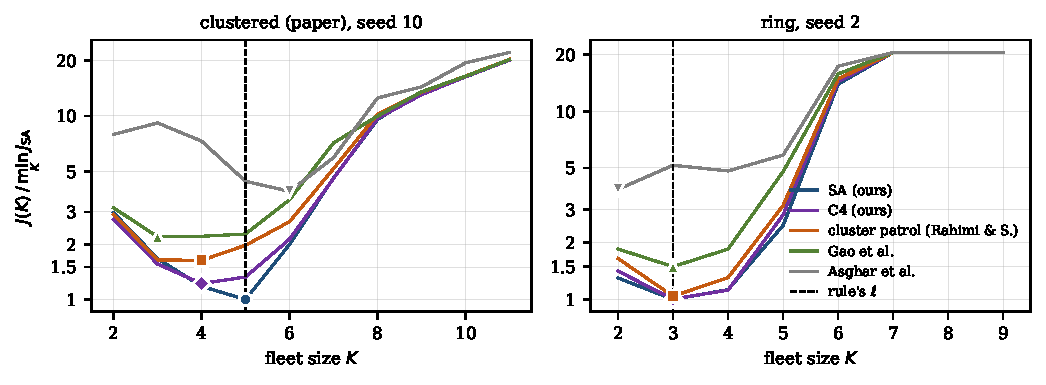
\includegraphics[width=.82\linewidth]{figs/fig_five}
\caption{Objective against fleet size under all five planners on two held-out deployments ($M=100$, $\Emax=1.5$~MJ), each curve divided by the annealer's minimum on the same deployment; markers at each planner's own optimum, dashed line at the rule's $\ell$. The deployments were fixed before the Gao et al.\ and Asghar et al.\ curves were seen: among the $M=100$, 1.5~MJ deployments, the one in each family whose C4-versus-cluster-patrol difference is closest to the median over the whole family (clustered: seed 10; ring: seed 2). On the clustered deployment the optima spread from 3 to 6 around $\ell=5$; on the ring every planner but Asghar et al.\ reaches its optimum at $\ell=3$. The levels differ several-fold.}
\label{fig:five}
\end{figure*}

\begin{table}[t]\centering
\footnotesize\setlength{\tabcolsep}{3pt}
\caption{C4 against four published methods on the 216 held-out deployments: median of $J^{\star}_{\mathrm{C4}}/J^{\star}_{X}-1$ at each planner's own optimum, with 95\% bootstrap interval, and deployments where C4 is lower. Last column: at the rule's fleet size $\ell$ instead.}
\label{tab:published}
\resizebox{\columnwidth}{!}{%
\begin{tabular}{llrrr}
\toprule
method $X$ & family & own optimum & C4 lower & at $K=\ell$\\
\midrule
cluster patrol \cite{rahimi2024graph} & paper & $-24.7\%$ $[-26.7,-19.0]$ & 72/72 & $-26.6\%$\\
 & core & $-10.3\%$ $[-12.0,-9.3]$ & 72/72 & $-10.4\%$\\
 & ring & $-5.9\%$ $[-7.3,-3.3]$ & 61/72 & $-3.1\%$\\
\midrule
Gao et al.\ \cite{gao2023aoi} & paper & $-43.8\%$ $[-46.1,-42.2]$ & 72/72 & $-49.3\%$\\
 & core & $-20.9\%$ $[-24.2,-18.2]$ & 72/72 & $-21.2\%$\\
 & ring & $-34.7\%$ $[-36.9,-32.2]$ & 72/72 & $-36.5\%$\\
\midrule
Asghar et al.\ \cite{asghar2025persistent} & paper & $-63.5\%$ $[-66.6,-61.8]$ & 72/72 & $-71.4\%$\\
 & core & $-57.0\%$ $[-58.7,-54.2]$ & 72/72 & $-62.2\%$\\
 & ring & $-67.5\%$ $[-70.5,-63.7]$ & 72/72 & $-69.4\%$\\
\midrule
Liu et al.\ \cite{liu2022aoi} & paper & $-9.3\%$ $[-13.1,-6.5]$ & 61/72 & $-9.3\%$\\
 & core & $-10.9\%$ $[-11.6,-8.6]$ & 72/72 & $-11.5\%$\\
 & ring & $-4.8\%$ $[-6.7,-1.7]$ & 50/72 & $-2.4\%$\\
\bottomrule
\end{tabular}%
}
\end{table}

\textit{A genetic-algorithm planner from IEEE IoT-J.} The strongest published method we found is the multi-population genetic algorithm of Liu et al.\ \cite{liu2022aoi}, which assigns sensors to UAVs and orders their tours jointly. We dropped the parts our model has no counterpart for (users, the interaction point, collision avoidance), treated each UAV's chromosome segment as its territory and repeating visit sequence, cut into energy-feasible sorties at launch as for the cluster patrol, and replaced its single-mission fitness by our time-average weighted age, evaluated on the same planner-side surrogate as C4; the published operators and settings are kept (8 populations of 60, 100 generations). The comparison with C4 was registered before the full run and uses the same union grid and extension rule as the other methods. Thirty-six of the 216 deployments ($M=50$, 1.5~MJ) had been seen in an earlier implementation study, and a first full run that executed our annealer under the wrong planner name was discarded before any statistic was computed. Liu et al.'s method is the strongest published baseline: the cluster patrol's own-optimum $J$ is a median $5\%$ higher, Gao et al.'s $45\%$ and Asghar et al.'s $134\%$, and our annealer's is $42\%$ higher on the core layout though $11\%$ lower on clustered fields. C4 is still lower in every family (Table~\ref{tab:published}): by a median $9.3\%$ on clustered fields, $10.9\%$ on the core layout and $4.8\%$ on the ring (50 of 72 deployments), $8.7\%$ overall (183 of 216), and by $7.1\%$ on the 36 previously seen deployments against $9.0\%$ on the rest. The rule predicts its optimum about as well as C4's (within one UAV in $86\%$ of deployments, $91\%$ where the design-time test passes), and sizing its fleet with $\ell$ costs a median $0.0\%$ of AoI.

\textit{A learned baseline, not reproduced.} We also attempted the multi-agent DRL method DRL-UCS($\mathrm{AoI}_{\mathrm{th}}$) \cite{wang2024drlucs}, using the authors' released code and hyperparameters, ported to current libraries (compatibility fixes only) and to our operating model: 5~s decision slots, our energy and depot model, and information restricted as for every other planner. The reproduction is incomplete. On the authors' own Beijing setting, at $10^7$ training steps (the released configuration uses $10^8$; the paper reports convergence near $10^7$), our run reached a threshold AoI of $52.5$ against the reported $26.8$. In our setting, with the same budget, the learned policy did not learn the task. With a 50~m collection radius the deterministic policy served at most 1 of 50 sensors (5 with sampled actions). With a 200~m radius, chosen on a pilot seed by a rule fixed in advance and applied to every planner, the deterministic policy served 2 of 50 sensors and the stochastic one 16; in that setting its AoI was about $20$ times the clustering baseline's. Two causes are plausible and we cannot separate them. One is reward sparsity: our field has about $0.3$ sensors per km$^2$ with collection at the sensor, against $7.6$ points of interest per km$^2$ in the original Beijing setting (244 over $32.1$~km$^2$), where a UAV collects from nearby points rather than only at each one, and the policy converges to repeatedly draining the sensors nearest the depot. The other is our port, given the incomplete reproduction on the authors' own setting. We therefore report no DRL comparison; whether a larger training budget or a faithful reproduction would close the gap is left open.

\begin{figure*}[t]\centering
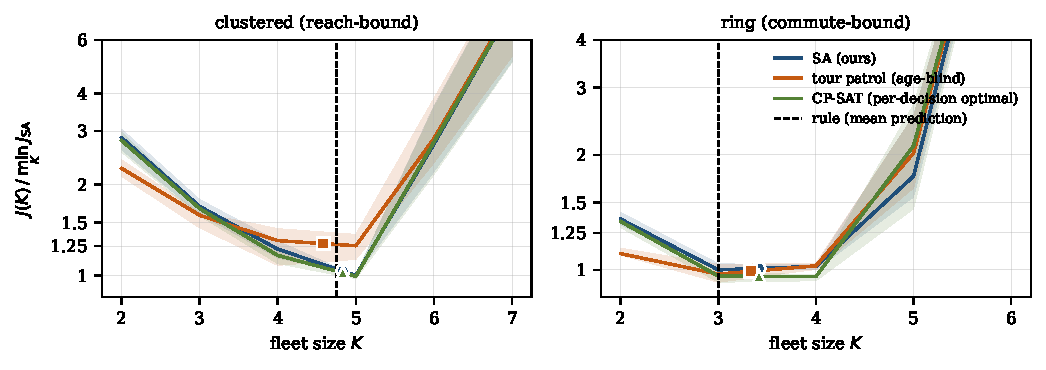
\includegraphics[width=.82\linewidth]{figs/fig_planners}
\caption{Objective against fleet size under three planners, $M=40$, $\Emax=1.5$~MJ: median over 12 instances of $J(K)$ divided by the annealer's minimum on the same instance, with interquartile bands. Normalising by one planner's minimum keeps the level differences visible. Markers: mean over instances of each planner's own optimum; dashed line: mean point prediction of the rule. The curves sit at different heights but reach their minimum at the same fleet size. On the ring the objective is nearly flat between $K=3$ and $4$ under every planner.}
\label{fig:planners}
\end{figure*}

\textit{Why the patrol wins on the ring.} Writing the weighted age at the realised visit frequencies $f_i$ and inter-visit variability $\mathrm{CV}_i$ as $J_2=\sum_i w_i(1+\mathrm{CV}_i^2)/(2f_i)$ and factoring it as $J_0\,E_{\mathrm{alloc}}\,E_{\mathrm{reg}}$, with $J_0=(\sum_i\sqrt{w_i})^2/2\Gam$ the ideal square-root allocation at the realised total rate, $E_{\mathrm{alloc}}=\sum_i w_i/(2f_i)\,/\,J_0$ and $E_{\mathrm{reg}}=J_2/\sum_i w_i/(2f_i)$, reproduces the simulator's measured age objective to within $0.6\%$ on 18 of the 20 runs we decomposed, as it must (the other two, one core instance at $K=6$, strand the outlier, whose age the interval statistics cannot include): for any visit sequence the time average of $t-t^{\mathrm{last}}_i$ is $(1+\mathrm{CV}_i^2)/(2f_i)$ with $\mathrm{CV}_i$ and $f_i$ from the same intervals, so this checks the bookkeeping (edge intervals aside), not the visit-frequency model, and it does not test whether the realised frequencies are optimal. Applied to the ring ($M=100$, 3~MJ, $K=4,6,8$, two seeds), it attributes the tour patrol's advantage almost entirely to the visit rate $\Gam$: the product of the three factors matches the measured ratio of objectives to within $3.3\%$, the rate factor tracks it in every instance, allocation favours the annealer by $1.5$--$4.7\%$ as expected of a policy that ignores priorities, and regularity is secondary, ranging from a $0.9\%$ loss to a $4.8\%$ gain for the patrol and favouring it mainly at larger $K$. The rate difference comes from shorter hops: at $K=4$ the patrol's inter-stop travel is $32.8$~s against the annealer's $42.5$~s, because consecutive stops on a tour are neighbours. We note the scope: this decomposition covers one cell and a two-run check at 1.5~MJ.

\textit{Better decisions do not monotonically improve the horizon.} The CP-SAT planner makes the point directly. Tripling its search budget raises the share of proven-optimal decisions per run on the ring from $0.67$--$0.99$ to $0.87$--$1.00$ at $K=2$--$4$, but changes $J$ by between $-9.2\%$ and $+7.9\%$ with a median of zero; tripling again, which proves $99.8\%$ of decisions optimal, changes two of six runs by $+0.9\%$ and $-1.0\%$ and leaves the other four bit-identical. A per-decision solution that is better, or even exact, changes the state the next decision starts from, and the rolling-horizon objective is myopic. Per-decision optimality is therefore not horizon optimality, and no per-decision solver, however exact, is a ground-truth oracle for $J$.

\textit{Resolution.} That sensitivity sets how finely the ring optimum can be resolved. At $M=40$, the cheaper fleet one UAV off the optimum costs a median $3.2\%$ in $J$ on the ring against $22\%$ on clustered fields, so a perturbation of a few percent in $J$ can move the argmin by one. At CP-SAT's default budget the ring argmin was biased upward for exactly this reason (exact agreement with the annealer $0.50$); at a threefold budget it rises to $0.67$, and a further threefold budget leaves the argmin unchanged on every instance checked, so the reported ring figures use the converged budget. Even then four instances differ from the annealer by one UAV, with the neighbouring fleet size $1.0$--$3.6\%$ worse under CP-SAT and 89--100\% of the decisions at those fleet sizes proven optimal. On commute-bound fields one-UAV resolution is therefore both what the measurement supports and all an operator needs.

\textit{Where the planners disagree.} The finite-window core regime is the exception, and it is instructive. At core $M=200$, 3~MJ, the tour patrol's optimum is $27.67$ against the annealer's $28.42$, both far above the rule's $10.33$: the stranding mechanism of Proposition~\ref{prop:strand} is not specific to the annealer, although how far it goes is planner-dependent (Section~\ref{sec:disc}). At 1.5~MJ the tour patrol places it at $11.00$ against $13.67$, within one UAV in only two instances of twelve. Once abandoning a peripheral sensor pays, the optimum balances that sensor's age against the service the rest of the field receives, and the second term depends on how well the planner serves the shrinking reachable set. The mechanism transfers; its precise location does not.

\subsection{Value of event-state information}\label{sec:eval:info}
The reach bracket holds for any routing policy; the commute branch enters through the rate curve the policy induces. We measure the value of one additional information channel a policy can exploit beyond the age vector: explicit knowledge of where events are live. On paired instances at $K=4$ (the rule's fleet size in 9 of 12) we compare the event-blind planner with the kernel-belief planner, and with the prior-rates planner to separate the kernel planner's two ingredients, across event correlation $q$ and event lifetime $\bar\tau$ (Table~\ref{tab:info}).

\begin{table}[t]\centering
\footnotesize\setlength{\tabcolsep}{3pt}
\caption{Kernel belief versus event-blind planner, paired over 12 instances, paper, $M=100$, $\Emax=1.5$~MJ, $K=4$, per-leg SA. $\Delta$catch is the relative change in the fraction of event episodes (overlapping firings merged) that are caught.}
\label{tab:info}
\resizebox{\columnwidth}{!}{%
\begin{tabular}{llrrrrl}
\toprule
$\bar\tau$ & $q$ & $\Delta J$ & $\Delta J_{\mathrm{age}}$ & $\Delta J_{\mathrm{event}}$ & $\Delta$catch (rel.) & sign test\\
\midrule
67.5 min & 0 & $-2.3\%$ & $+1.2\%$ & $-8.2\%$ & $+0.8\%$ & n.s.\\
67.5 min & 0.5 & $-1.9\%$ & $+1.8\%$ & $-8.3\%$ & $+0.4\%$ & n.s.\\
67.5 min & 1 & $-2.8\%$ & $+1.5\%$ & $-9.9\%$ & $+0.7\%$ & n.s.\\
15 min & 1 & $+3.6\%$ & $+5.5\%$ & $-4.2\%$ & $+6.3\%$ & worse, $p=.006$\\
5 min & 1 & $+2.8\%$ & $+3.0\%$ & $-1.2\%$ & $+10.0\%$ & worse, $p=.006$\\
\bottomrule
\end{tabular}%
}
\end{table}

Three things follow. The gain from belief does not depend on $q$: spatial correlation carries no exploitable information at these parameters. The $2$--$3\%$ at long lifetimes, not significant, comes from the kernel's use of observations rather than from the prior rates: the prior-rates planner alone is $2.4$--$3.4\%$ \emph{worse} (9 of 12 instances, n.s.), because weighting sensors by their prior event probability costs more in buffer age ($+9.6\%$) than it saves in event age. For events comparable in duration to a sortie, belief is harmful: the planner catches more events but sacrifices freshness, and the event term it protects is only $4$--$20\%$ of $J$ because most short events expire before any UAV can reach them. And $K^{\star}$ is unchanged under correlated events with the kernel planner (12/12 agreement).

What this does and does not bound is worth stating precisely. It bounds \emph{one} channel of possible advantage---explicit knowledge of event state---within the information structure and event model of Section~\ref{sec:model}: at these parameters that channel is worth $2$--$3\%$ (not significant) and is negative for short-lived events. It does not bound advantages available from better sequencing, better sensor-to-UAV partitioning, or non-myopic energy use across sorties. The per-decision certificates of Section~\ref{sec:planner:cert} and the CP-SAT comparison of Section~\ref{sec:eval:baseline} close part of that remaining gap, but they reach $M=40$, not the headline configuration, and set-orienteering hardness grows quickly with $M$; we therefore do not claim the planner is near-optimal at $M=400$. The defensible statement is that explicit event-state information adds little over an age-based index at the fleet-size optimum, not that a learned policy cannot help.

\section{Discussion and Limitations}\label{sec:disc}
\textit{Using the rule.} Algorithm~\ref{alg:procedure} collects the pre-deployment procedure. Every input is known before the fleet flies; nothing in it requires a simulation, a pilot sortie or a fleet sweep unless the design-time test flags the field. It uses the robust reach cap throughout, and when the test flags a field it sweeps upward from $K_0$ under the extension rule of Section~\ref{sec:eval:setup}, capped at the $K_{\max}$ of \eqref{eq:window_apriori}, rather than stopping at Result~\ref{thm:law}'s $K_R$, whose coverage was validated with measured commute inputs; with ex-ante inputs $K_{\max}$ can be several hundred, so in practice the extension rule ends the sweep; the flight-only alternative of Section~\ref{sec:eval:law} is an operational choice that depends on the interruptions a deployment must tolerate, and is deliberately left out of the procedure.

\begin{algorithm2e}[t]
\caption{Pre-deployment fleet sizing}\label{alg:procedure}
\DontPrintSemicolon
\KwIn{sensor positions $x_i$, depot $x_0$, weights $w_i$, nominal rates $\lambda_i$; airframe $v,\Pf,\Ph,\Ru,B$; inventory $U$; window $T_b,T$}
\KwOut{a fleet size, or an interval to sweep}
$r_i\gets\|x_i-x_0\|$, $\rmax\gets\max_i r_i$\;
$\Kr\gets vU/(2\Pf\rmax+v\Ph B/\Ru)$ \tcp*{robust reach cap, \eqref{eq:Kreach}}
at $K=\lfloor0.5\Kr\rfloor$: $\hat\rc$ from the radial order statistic, $\hat{\Pbar}$ from hover conservation; $\hat K_{\mathrm{commute}}\gets\Kc(\hat\rc,\hat{\Pbar})$ \tcp*{Sec.~\ref{sec:eval:exante}}
$K_0\gets\lfloor\Kr\rfloor$, $\ell\gets\min(K_0,\mathrm{round}\,\hat K_{\mathrm{commute}})$\;
\lIf{$\ell<K_0$}{\Return $\ell$ \tcp*[h]{commute-bound}}
\lIf{\eqref{eq:window_apriori} holds, with $(\hat\rc,\hat{\Pbar})$}{\Return $K_0$ \tcp*[h]{reach-bound}}
sweep upward from $K_0$ until the three largest $K$ each exceed $1.5\times$ the minimum, at most to $K_{\max}$, and \Return the best \tcp*{stranding may pay}
\end{algorithm2e}

\textit{Duty cycling.} Proposition~\ref{prop:duty} shows the rule sizes the airborne fleet $K\delta$ rather than the airframe count, so an operator cannot evade the reach cap by buying more UAVs and flying them less. The corollary is that the two are interchangeable for freshness, and, under Proposition~\ref{prop:duty}(iii), airframes beyond $\lceil K^{\star}\rceil$ are only useful as redundancy.

\textit{Scope of the energy model.} The shared-budget assumption of Remark~\ref{rem:budget} is what makes fleet size non-monotone, and it is an assumption about a shared energy \emph{stock}; a fixed charging \emph{rate} bounds the airborne count by a different mechanism that we do not model; under independent per-airframe batteries with no other shared bottleneck neither cap yields a finite optimum, since the reach radius no longer shrinks with $K$ and the fleet visit rate is monotone increasing (Remark~\ref{rem:budget}). Equal allocation (Remark~\ref{rem:equal}) is likewise a modelling choice rather than an optimum; sizing one UAV's share for the peripheral sensor removes the stranding regime in the two core cells tested (Sec.~\ref{sec:eval:fail}), and the general allocation problem remains open.

\textit{Modelling.} Results rest on a single simulator and on our placement and energy models. The reachability bracket is geometric and transfers to any field shape and depot location through $\rmax$, but the full rule does so only where a field-average commute radius represents the field: with an off-centre depot the ring layout's far side binds through commute cost and the rule is one UAV too high (Sec.~\ref{sec:eval:depot}); the commute cap and the boundary transfer with the realised $(\rc,\Pbar)$ but the closed form's constant-cost assumption does not, as the 3~MJ ring cells show. Wind and altitude changes are not modelled; depot position is tested in Section~\ref{sec:eval:depot}. Validation on a real sensor layout is the natural next step.

\textit{Objective.} Age is reset at collection, not delivery. Deconfliction near the depot is not modelled; asynchronous relaunch reduces near-depot congestion, but at the largest fleets here (core, 3~MJ, optima near 28) it may matter.

\textit{Planner dependence.} The reach bracket holds for any routing policy; which point inside it a planner sustains does not. The commute branch enters through the rate curve a policy induces, and Section~\ref{sec:eval:baseline} measures how much that matters: little for the location of the optimum in most regimes, a great deal for the level of $J$, and decisively in the finite-window core regime. At core $M=200$, 1.5~MJ, every planner strands the outlier in most deployments (9 to 12 of 12); at 3~MJ the optimum lies above the reach cap by $18.1$ UAVs for the annealer, $17.3$ for the tour patrol and $11.9$ for Asghar et al., but by $6.5$ for C4 and Liu et al.\ and $5.3$ for the cluster patrol (which strand in 4 to 6 of 12 deployments) and by $0.25$ for Gao et al., which never strands. On commute-bound fields the objective is flat enough near the optimum ($3.2\%$ for the cheaper neighbouring fleet size at $M=40$) that no planner we tested resolves it more finely than one UAV at $M=40$.

\textit{Statistics.} The per-instance statistic is what a step-function rule requires; population means blur it. Agreement rates and regret are the primary evidence. Aggregate agreement rates have 95\% intervals from a bootstrap that resamples instances within each cell, keeping the cell design fixed (10{,}000 replicates; exact Clopper--Pearson intervals where a rate is $0$ or $1$); regret is reported by its quantiles. Per-cell intervals are Clopper--Pearson; with 12 instances each they are wide --- six agreements in twelve gives $[21,79]\%$ --- and are given in the supplementary data rather than in Table~\ref{tab:law}; the per-cell sign tests are descriptive, reported per cell without correction for multiplicity, and the lower-side test is at $p<.001$ in 19 of the 20 primary cells; the exception is paper $M=50$ ($p=.006$).

\section{Conclusion}\label{sec:conc}
The number of UAVs a continuously operating data-collection fleet should keep airborne is bounded by two physically distinct mechanisms, and the boundary $\rmax/\rc=1+\sqrt{\Pbar/\Pf}$ predicts which one binds. The reach cap is a feasibility statement about the farthest sensor, exact as a bracket between its full-buffer and flight-only limits, and duty cycling relocates it to the airborne count rather than removing it (Proposition~\ref{prop:duty}). The commute branch rests on an exact allocation principle --- cost-weighted square-root frequencies, under which minimising weighted age is equivalent to maximising the fleet's visit rate, which under a fixed normalised cost profile is proportional to productive energy per unit time divided by the mean energy a visit costs (Proposition~\ref{prop:sqrt}) --- together with a first-order closed form that approximates it. We are explicit about which is which: in the layout family where the closed form misses by two UAVs, the principle holds within one UAV in every instance and exactly for the cell-mean curves, and the error is traceable to a single measurable quantity, the $K$-dependent inter-stop travel time that Proposition~\ref{prop:tau} isolates from the dwell time it proves irrelevant.

The rule was validated per instance across three layout families, four sensor counts, three budgets and five field sizes. Its failure modes were characterised rather than averaged over: a stranding condition prices when exceeding the coverage bound is worthwhile, and a pre-deployment criterion, computable from the site survey and known system parameters, flags in advance the deployments where the reach branch may not govern within the operating window. Fleet coordination through shared commitments is a prerequisite for the measurement rather than a refinement, costing a factor of $2.7$--$2.9$ in the objective and two-thirds of a UAV in the mean optimum when omitted. Finally, explicit event-state information adds little over an age-based index at the optimum within the event model studied. The optimum itself largely survives a change of planner: an age-blind tour patrol and a planner that proves almost all its decisions optimal locate it within one UAV of ours in most deployments while achieving materially different AoI, and the rule predicts their optima about as well as it predicts ours. The exception is instructive. Where stranding a peripheral sensor pays, every planner we tested places the optimum above the reach cap in most deployments at 1.5~MJ, and all but one do at 3~MJ, but the precise point is planner-dependent; the mechanism is structural, its location is not.

\appendices
\section{Derivation of the commute cap}\label{app:commute}
With $a=\Pf t_c$ and $b=t_c(\Pbar-\Pf)$, \eqref{eq:R} is $\Gam\propto f(K)=K(U-aK)/(U+bK)$. Then $f'(K)\propto(U-2aK)(U+bK)-b(UK-aK^2)=U^2-2aUK-abK^2$, whose positive root is $K=U(\sqrt{a^2+ab}-a)/(ab)=\frac{U}{a}\cdot\frac{\sqrt{1+b/a}-1}{b/a}$. Since $b/a=\Pbar/\Pf-1$, $\sqrt{1+b/a}=\sqrt{\Pbar/\Pf}$ and $K=\frac{U}{a(1+\sqrt{\Pbar/\Pf})}=\frac{U}{t_c(\Pf+\sqrt{\Pf\Pbar})}$, which is \eqref{eq:Kcommute}. With sublinear yield $n=c(\Eu-a)^{\alpha}$ the maximiser of $Kn/(t_c+n\tau_s)$ has no closed form; it is computed numerically from measured $(c,\alpha,\tau_s)$, and in the fitted ring cells of Table~\ref{tab:alpha} it lies at or above \eqref{eq:Kcommute}; we have not shown that this holds for $\alpha<1$ in general.

\section{Supplementary diagnostics}\label{app:diag}
\textit{Choice of estimator.} For transparency, the alternatives and what they would report: taking the argmin of mean $J$ per cell gives exact agreement $0.489$ and within-one $0.735$; of median $J$, $0.504$ and $0.816$; of mean relative regret $J(K)/J(K^{\star}_{\mathrm{inst}})$, $0.489$ and $0.735$; against $0.559$ and $0.798$ for the per-instance estimator we adopt. The four disagree on the summarised optimum in 8 of 24 cells. No cell-level alternative matches the per-instance estimator on exact agreement, and the robust ones gain little over the plain mean there (the median does better on within-one, $0.816$, than both the mean and the per-instance estimator), so the gap in exact agreement is not an outlier effect; it is the granularity mismatch above. A practitioner sizing a fleet for one deployment faces the per-instance question; an operator choosing a single $K$ for a portfolio of future deployments faces the aggregate one, and should then also compare against a rule evaluated at the population geometry rather than at each instance's.

\textit{A fitted commute exponent.} Fitting $n=c(\Eu-\Pf t_c)^{\alpha}$ on the stranding-free rows and re-maximising recovers part of the missing UAVs (Table~\ref{tab:alpha}): the corrected form predicts 7 where the closed form predicts 6 in the $M=50$ and $M=100$ 3~MJ ring cells, against measured optima of $8.50$ and $7.92$; at $M=200$ and at 1.5~MJ both forms agree. We report this as a diagnosis rather than adopting it as the rule, for a reason that is worth stating plainly: $\alpha$ is \emph{fitted}, and a rule whose claim is that it contains no fitted constants should not acquire one to recover part of two cells. Deriving $\alpha$ from the layout geometry --- as Proposition~\ref{prop:eta} derives $\eta$ --- would make the commute branch both parameter-free and accurate, and is the natural next piece of theory. We tested the most promising candidate derivation and report it as a negative result, because the way it fails is informative. If the planner's marginal insertion costs $X$ have a locally $d$-dimensional law $F_X(x)\sim Ax^{d}$, then cost-aware selection at a value-per-energy threshold gives $n\propto\theta^{-d}$ and $E_{\mathrm{hop}}\propto\theta^{-(d+1)}$, hence $E_{\mathrm{hop}}\propto n^{(d+1)/d}$ and $\alpha_{\mathrm{geom}}=d/(d+1)=2/3$ for a locally planar layout --- strikingly close to the $0.66$ and $0.72$ observed. Per-sortie regression refutes it. Over the post-burn-in sorties with at least two stops of the stranding-free runs in the three 3~MJ ring cells (seeds 1--4, every swept $K$; about $4{,}500$--$4{,}900$ sorties per cell, 95\% intervals by bootstrap over runs), $\log E_{\mathrm{hop}}$ on $\log n$ gives slopes $1.06$, $0.92$ and $0.93$ ($[0.88,1.21]$, $[0.66,1.06]$, $[0.80,0.99]$): all exclude the predicted $1.5$, and marginal stops are no dearer in hop energy than average ones, so the mechanism is absent.

The decomposition into hop and hover energy then locates the difficulty, and it is not where the fitted exponent suggests. Hover energy per sortie scales roughly linearly in $n$ on the same sample ($\beta_{\mathrm{hov}}=1.08$, $0.94$, $0.87$), and its level is what the conservation argument of Proposition~\ref{prop:tau} predicts: a fixed total hovering requirement $H$ shared over a fleet visit rate $\Gam(K)$ gives $E_{\mathrm{hov}}/n=\Ph H/\Gam(K)$, which the measured hover energy per stop matches to a factor of $0.99\pm0.01$ across the three cells. But hover is only $7$--$24\%$ of productive energy here, too small a share to produce the aggregate exponent. Decisively, \emph{measured} per-sortie productive energy grows at most linearly in $n$ ($\beta_p=1.05$, $0.90$, $0.91$; $[0.88,1.17]$, $[0.70,1.01]$, $[0.81,0.97]$) while the aggregate fit implies $1/\alpha=1.51$, $1.39$, $1.19$. The two disagree. The resolution is that $\Eu-\Pf t_c$ is a budget proxy, not energy actually spent: sorties do not exhaust their allowance and $t_c$ is a cell-level mean. We therefore conclude that $\alpha$ is an elasticity of the closed loop --- routing geometry, visit-rate feedback and backlog state compressed into one number --- rather than a geometric constant of the layout, and we do not attempt to derive it.

\textit{The ring miss lies in the stop-count model, not the principle.} The commute principle itself holds in these cells: the fleet size that maximises the \emph{measured} visit rate $K\bar n/\bar T_s$ lies within one UAV of the AoI optimum in every instance of every ring cell, the three 3~MJ cells included. The principle is not specific to our planner: over all ring deployments the same holds for the tour patrol in every instance, and in $97\%$ of deployments for C4, $92\%$ for the cluster patrol and Liu et al., $83\%$ for Gao et al.\ and $71\%$ for Asghar et al., whose class-based allocation leaves some UAVs nearly idle. What fails is the stop-count model. Calibrating it from measurement rather than fitting it to the outcome --- estimating the budget elasticity of the stop count from each planner's two smallest stranding-free swept fleet sizes, as pilot runs, and re-maximising the visit rate --- recovers the annealer's optimum within one UAV in 65 of 72 ring deployments, against 49 for the closed form, and in $58$, $83$ and $100\%$ of the three 3~MJ cells against $0$, $8$ and $100\%$. It does not help every planner: on the same 36 deployments within-one agreement rises from $50\%$ to $72\%$ for Gao et al.\ and from $72\%$ to $86\%$ for Liu et al., is unchanged for the cluster patrol ($81\%$ and $83\%$), and falls from $75\%$ to $58\%$ for C4 and from $94\%$ to $31\%$ for Asghar et al. The planners' optima in these cells are spread over several UAVs --- mean $6.7$--$8.5$ for the annealer, $5.1$--$7.8$ for C4, $5.0$--$7.1$ for the cluster patrol, $5.2$--$7.7$ for Liu et al., $6.6$--$6.9$ for Asghar et al.\ and $4.4$--$5.1$ for Gao et al.\ --- and the closed form's $6$ lies inside that spread, while the tour and sweep patrols miss like the annealer (optima $8.0$, $7.2$, $5.9$ and $8.0$, $7.0$, $5.7$). We therefore keep the uncorrected closed form, which is the planner-independent prediction, and read the ring failure family as a property of how the realised stop count scales with the budget, which the closed form's constant per-stop cost cannot capture and which the annealer shares with both age-blind patrols.

\begin{table}[t]\centering
\caption{Diagnosing the commute branch: measured optimum against the closed form ($\alpha=1$) and against a fitted sublinear stop count. Ring layout.}
\label{tab:alpha}
\small
\begin{tabular}{lcccc}
\toprule
cell & measured & $\alpha=1$ & $\alpha$-corrected & fitted $\alpha$\\
\midrule
$M{=}50$, 3~MJ & 8.50 & 6 & \textbf{7} & 0.66\\
$M{=}100$, 3~MJ & 7.92 & 6 & \textbf{7} & 0.72\\
$M{=}200$, 3~MJ & 6.67 & \textbf{6} & \textbf{6} & 0.84\\
$M{=}100$, 1.5~MJ & 3.00 & \textbf{3} & \textbf{3} & 0.88\\
\bottomrule
\end{tabular}
\end{table}

\section{Reproducibility}
Every number in this paper is traceable to rows of the released CSV files, each stamped with the simulator version. The main runs are keyed by (layout, $M$, $\Emax$, $L$, $K$, seed, planner, coordination, replanning, diversion, $q$, belief, $\bar\tau$, window, and the depot position or energy split where these vary); the secondary files carry their own keys: the battery-mass runs add a mass-model tag, the grounding test (annealer only) is keyed by instance, fleet-size choice and grounding length, and the regularity and per-sortie files by planner, instance, $K$ and, for the latter, sortie. All results come from version 2.2 of the simulator. It corrects faults of the version used during development that changed $J$ by amounts depending on $K$: a UAV that reached a stop it could not afford was charged nothing for that leg and flew home from its previous stop; a dwell advanced the shared clock past other UAVs' pending events, which were then processed late; an event firing at a sensor whose event was still live replaced it instead of extending it; and a mid-leg diversion neither charged the abandoned leg nor cancelled the pending arrival. Version 2.2 also adds the departure check of Section~\ref{sec:model} and per-sensor event streams (Section~\ref{sec:eval:setup}), and weights diversion targets as the planner weights its candidates. The earlier behaviour is retained behind switches and reproduces its reference values exactly; every simulation in this paper, including the registered planner comparisons, was rerun once on version 2.2 with no planner setting changed (C4's and Liu et al.'s design surrogates share the corrected energy accounting). A single command, \texttt{python reproduce\_v2.py results\_v2}, checks the version stamp of every file, reports every sweep that does not meet the extension rule (the extension is applied to every planner on the primary grid, to the annealer's extra cells and to the depot studies; for the $M=40$, battery-mass and reserved-share sweeps it reports whether the optimum is interior and whether the $1.5\times$ condition holds), and regenerates the tables, statistics, intervals and figures from the recorded runs without running the simulator. The per-decision certification and CP-SAT probes, the decision-time benchmark, Fig.~\ref{fig:teaser} and the $\eta$ Monte Carlo come from their own scripts, listed with their commands in the repository; the bootstrap uses fixed seeds, so the outputs are identical run to run. Code and data: \url{https://github.com/Hvir704/Trajectory_Optimisation_in_Multi_UAV_Network}.

\bibliographystyle{IEEEtran}
\bibliography{IEEEabrv,refs}
\end{document}
